% Copyright 2022 Haute école d'ingénierie et d'architecture de Fribourg
%
% Licensed under the Apache License, Version 2.0 (the "License");
% you may not use this file except in compliance with the License.
% You may obtain a copy of the License at
%
% http://www.apache.org/licenses/LICENSE-2.0
%
% Unless required by applicable law or agreed to in writing, software
% distributed under the License is distributed on an "AS IS" BASIS,
% WITHOUT WARRANTIES OR CONDITIONS OF ANY KIND, either express or implied.
% See the License for the specific language governing permissions and
% limitations under the License.

% =============================================================================
% | HES-SO//Master - Thesis project report template                           |
% |                                                                           |
% | Originally based on the EPFL template, with many adjustments             |
% =============================================================================

% Document settings
\documentclass[a4paper,11pt,fleqn]{book}
\usepackage[utf8]{inputenc}
\usepackage[T1]{fontenc}
\usepackage[english]{babel}



% -----------------------------------------------------------------------------
% Preamble
% -----------------------------------------------------------------------------
% =============================================================================
% | Thesis metadata                                                           |
% =============================================================================

% Thesis info
\newcommand{\ThesisTitle}{GPU optimization - Celeritas}
\newcommand{\ThesisSubject}{}
\newcommand{\Orientation}{Information and communication systems (ICS) }
\newcommand{\Keywords}{}
\newcommand{\Keywordsfr}{}
\newcommand{\reportVersion}{v0.1}
\newcommand{\specificationVersion}{v1.3}

% Author
\newcommand{\AuthorFirstName}{Simon }
\newcommand{\AuthorLastName}{Barras}
\newcommand{\Author}{\AuthorFirstName \AuthorLastName}

% Advisor
\newcommand{\AdvisorFirstName}{Frédéric }
\newcommand{\AdvisorLastName}{Bapst}
\newcommand{\AdvisorSchool}{HEIA-FR}
\newcommand{\Advisor}{Prof. \AdvisorFirstName \AdvisorLastName}
\newcommand{\AdvisorTwoFirstName}{Jean }
\newcommand{\AdvisorTwoLastName}{Hennebert}
\newcommand{\AdvisorTwoSchool}{HEIA-FR}
\newcommand{\AdvisorTwo}{Prof. \AdvisorTwoFirstName \AdvisorTwoLastName}
\newcommand{\Expert}{Dr. Baptiste Wicht}

% Mendant
\newcommand{\Mendant}{\acrfull{lbl}\\ & Paolo Calafiura\\ & Julien Esseiva}

% Place (for date and place)
\newcommand{\Date}{\today}
\newcommand{\Place}{Berkeley, CA, USA}
         % your project data
% ==================
% Template settings
% ==================

% General tools
% -------------
\usepackage{etoolbox}
\usepackage{listings}

% Page style
% ----------
\usepackage[margin=3cm, left=3.5cm, right=3.5cm, twoside=false]{geometry}
\usepackage{fancyhdr}
\setlength{\headheight}{14pt}
\renewcommand{\sectionmark}[1]{\markright{\thesection\ #1}}
\pagestyle{fancy}

% Standard pages (inside chapters)
\fancyhf{}
\renewcommand{\headrulewidth}{0.4pt}
\renewcommand{\footrulewidth}{0.4pt}
\fancyhead[R]{\bfseries \nouppercase{\rightmark}}
\fancyhead[L]{\bfseries \nouppercase{\leftmark}}
\fancyfoot[L]{\Author \space - \ThesisTitle}
\fancyfoot[R]{\thepage}

% First page of chapters
\fancypagestyle{plain}{
	\fancyhf{}
	\renewcommand{\headrulewidth}{0pt}
	\fancyfoot[L]{\Author \space - \ThesisTitle}
	\fancyfoot[R]{\thepage}
}

% Imports for external PDFs
\fancypagestyle{addpagenumbersforpdfimports}{
	\fancyhead{}
	\renewcommand{\headrulewidth}{0pt}
	\fancyfoot{}
	\fancyfoot[R]{\thepage}
}

% Use empty style for page when clearing double pages
%\def\cleartoodd{%
%	\clearpage%
%	%\ifodd\value{page}\else\mbox{}\thispagestyle{empty}\newpage\fi%
%}

%\def\clearchap{%
%	\ifodd\value{page}\else\mbox{}\thispagestyle{empty}\fi%
%}

% \cleardoublepage replaced by \cleartoodd
%\let\origdoublepage\cleardoublepage
%\renewcommand{\cleardoublepage}{%
%	\cleartoodd%
%}

% Fonts
% -----

% Helvetica (Arial used in the MSE Word template)
\usepackage{helvet}
\usepackage{lmodern}
\usepackage[T1]{fontenc}


% Math
% ----
\usepackage{amsmath}  % better math

% Floats and figures
% ------------------
\usepackage{newfloat}          % floats
\usepackage[oneside]{caption}  % captions
\usepackage{subcaption}        % subcaptions
\usepackage[section]{placeins} % allows to put float barriers

% Float captions in italics, with the label in the margin
%\DeclareCaptionLabelFormat{title}{#1 #2}
%\DeclareCaptionLabelFormat{hangout}{\llap{#1 #2\hspace{5mm}}}
%\captionsetup{
%	format=hang,
%	labelformat=hangout,
%	singlelinecheck=false,
%	font={it}
%}

% Caption with a source for a figure
% TODO: improve this to use square brackets like the normal "caption"
\newcommand*{\captionsource}[3]{%
	\caption[{#1}]{%
		#2%

		\textbf{Source:} #3%
	}%
}

% Tables
% ------
\usepackage{booktabs} % much better tables
\usepackage{multirow} % allows to fuse rows
\usepackage{array}    % manipulate array
\usepackage{tabularx} % better tables

% Define new tabularx column types:
%  - R: streteched right-aligned
%  - C: stretched centered
%  - N: left aligned, specified space
\newcolumntype{R}{>{\raggedleft\arraybackslash}X}%
\newcolumntype{C}{>{\centering\arraybackslash}X}%
\newcolumntype{N}[1]{>{\raggedleft\arraybackslash}p{#1}}

% Set row height multiplicator to provide more breathing space
\renewcommand{\arraystretch}{1.3}

% Bibliography
% -------------------

% Use biber, with numeric style and no sorting (citation order)
\usepackage[
backend=biber,
style=numeric,
sorting=none,
bibencoding=auto
]{biblatex}
\addbibresource{bibliography.bib}


% Tables of contents, figures, tables and listings
% ------------------------------------------------
\usepackage{tocloft}
\newlistof{listing}{lol}{List of Listings}
\setcounter{tocdepth}{1} % Depth to 'section'
\setlength{\cftfigindent}{0pt}  % remove indentation from figures in lof
\setlength{\cftfignumwidth}{1cm}
\setlength{\cfttabindent}{0pt}  % remove indentation from tables in lot
\setlength{\cfttabnumwidth}{1cm}
\setlength{\cftlistingindent}{0pt}
\setlength{\cftlistingnumwidth}{1cm}

% Mini tables of contents
% -----------------------
\usepackage{minitoc}

% no "Contents" title
\mtcsettitle{minitoc}{Contents}

% Layout
\setlength{\mtcindent}{-0.5em}
\mtcsetoffset{minitoc}{-1em}

% Spacing above and below table
\mtcsetfeature{minitoc}{before}{\vspace{0.5cm}}
\mtcsetfeature{minitoc}{after}{\vspace{-0.25cm}}
\renewcommand{\mtifont}{\sffamily\bfseries\large}

% Colors & graphics
% -----------------
\usepackage[table]{xcolor}    % colors
\usepackage[pdftex]{graphicx} % graphics importing
\graphicspath{{02-main/figures/}}
\definecolor{gray80}{gray}{0.80}


% Code and syntax highlighting
% ----------------------------
\usepackage[newfloat]{minted}   % code highlighting
\newenvironment{code}{\captionsetup{type=listing}}{}

% Typography
% ----------
\usepackage{csquotes}                    % paragraph indentation and spacing
\usepackage[defaultlines=3,all]{nowidow} % avoid widows and orphans
\usepackage{microtype}                   % typographic improvements
\usepackage{parskip}                     % No indent and auto-space between paragraphs
\usepackage[super]{nth}
\usepackage{amsmath}

\usepackage{paralist}
\usepackage{enumitem}
\setlist{after=\vspace{\baselineskip}}

% Section and chapters headings
% -----------------------------
\usepackage[explicit]{titlesec} % titles formatting
%\usepackage{titletoc} % titles formatting in ToC etc
%\usepackage{sectsty}  % sectioning commands

% -- Chapters --
% Remove "Chapter N" and use a sans-serif font

% Set layout lengths
\setlength{\headheight}{8mm}
\setlength{\footskip}{1.5cm}
\addtolength{\textheight}{-.5cm}

\titlespacing{\chapter}{-5mm}{-10mm}{3mm}
\titlespacing{\section}{-5mm}{3mm}{2mm}
\titlespacing{\subsection}{-5mm}{2mm}{2mm}
\titlespacing{\subsubsection}{-5mm}{2mm}{1mm}


%\titleformat{\chapter}[block]
%{\Huge}
%{\thechapter\hspace{12pt}\textcolor{gray80}{|}\hspace{12pt}}
%{0pt}
%{\Huge\bfseries}

\titleformat{\chapter}{\Huge\bfseries}{\llap{\thechapter\hspace{12pt}\textcolor{gray80}{|}}}{0mm}{%
	\hfill\begin{minipage}[t]{\dimexpr\textwidth}\raggedright#1\end{minipage}%
}
\titleformat{\section}{\Large\bfseries}{\llap{\thesection}}{0mm}{%
	\hfill\begin{minipage}[t]{\dimexpr\textwidth}\raggedright#1\end{minipage}%
}
\titleformat{\subsection}{\large \bfseries}{\llap{\thesubsection}}{0mm}{%
	\hfill\begin{minipage}[t]{\dimexpr\textwidth}\raggedright#1\end{minipage}%
}
\titleformat{\subsubsection}{\bfseries}{\llap{\thesubsubsection}}{0mm}{%
	\hfill\begin{minipage}[t]{\dimexpr\textwidth}\raggedright#1\end{minipage}%
}

% Misc
% ------
\usepackage{lipsum}    % filler text
\usepackage{blindtext} % random text
\usepackage{lscape}    % easy landscape pages
\usepackage{pdflscape} % landscape pages for PDFs

% Allow email typesetting
\newcommand{\email}[1]{%
	\href{mailto:#1}{\textit{#1}}%
}

% References
% -----------
\usepackage{url}

% pdf metadata
\usepackage[
	pdfauthor={\Author},
	pdftitle={\ThesisTitle},
	pdfsubject={\ThesisSubject},
	pdfkeywords={\Keywords}
	pdfduplex=DuplexFlipLongEdge]{hyperref}

% Hyperlinks
\hypersetup{
	colorlinks=true,
	linkcolor=black,
	citecolor=black,
	filecolor=black,
	urlcolor=black,
}
\providecommand*{\listingautorefname}{Listing}


% % Glossary
% % --------
%\usepackage[xindy, toc, nonumberlist]{glossaries}
\usepackage[acronym]{glossaries}
\makeglossaries
\newacronym{heia}{HEIA-FR}{Haute Ecole d'Ingénierie et d'Architecture de Fribourg}

\newacronym{os}{OS}{Operating System}

\newacronym{gpu}{GPU}{Graphics Processing Unit}

\newacronym{cpu}{CPU}{Central Processing Unit}

\newacronym{cuda}{CUDA}{Compute Unified Device Architecture}

\newacronym{lbl}{LBNL}{Lawrence Berkeley National Laboratory}

\newacronym{ornl}{ORNL}{Oak Ridge National Laboratory}

\newacronym{anl}{ANL}{Argonne National Laboratory}

\newacronym{fnal}{FNAL}{Fermi National Accelerator Laboratory}

\newacronym{bnl}{BNL}{Brookhaven National Laboratory}

\newacronym{cern}{CERN}{European Organization for Nuclear Research}

\newacronym{lhc}{LHC}{Large Hadron Collider}

\newacronym{doe}{DOE}{Department of Energy}

\newacronym{smart}{SMART}{Specific, Measurable, Achievable, Relevant, Time-bound}

\newacronym{hpc}{HPC}{High Performance Computing}

\newacronym{nersc}{NERSC}{National Energy Research Scientific Computing Center}

\newacronym{atlas}{ATLAS}{A Toroidal LHC ApparatuS}

\newacronym{cms}{CMS}{Compact Muon Solenoid}

\newacronym{hep}{HEP}{High Energy Physics}

\newacronym{rkdp}{RKDP}{Runge Kutta Dormand Prince}

\newacronym{simd}{SIMD}{Single Instruction Multiple Data}

\newacronym{sisd}{SISD}{Single Instruction Single Data}

\newacronym{sm}{SM}{Streaming Multiprocessor}

\newacronym{sdk}{SDK}{Software Development Kit}

\newacronym{api}{API}{Application Programming Interface}

\newacronym{simt}{SIMT}{Single Instruction Multiple Thread}



\usepackage{tabularray}    % template settings
% ===========================================
% = Codestyles for minted syntax highlighting
% ===========================================


% How to use (replace 'java' with language name):
% - code blocks:
%     \begin{javacode}
%     CODE
%     \end{javacode}
% - files:
%     full: \javafile{PATH}
%     extract: \javafile[startline=x, endline=y]{PATH}

% c#
\newminted{csharp}{frame=single, framesep=6pt, breaklines=true, fontsize=\scriptsize}
\newmintedfile{csharp}{frame=single, framesep=6pt, breaklines=true,
fontsize=\scriptsize}

% Java
\newminted{java}{frame=single, framesep=6pt, breaklines=true, fontsize=\scriptsize}
\newmintedfile{java}{frame=single, framesep=6pt, breaklines=true,
fontsize=\scriptsize}

% JavaScript
\newminted{js}{frame=single, framesep=6pt, breaklines=true, fontsize=\scriptsize}
\newmintedfile{js}{frame=single, framesep=6pt, breaklines=true, fontsize=\scriptsize}

% Scala
\newminted{scala}{frame=single, framesep=6pt, breaklines=true, fontsize=\scriptsize}
\newmintedfile{scala}{frame=single, framesep=6pt, breaklines=true,
	fontsize=\scriptsize}

% Clojure
\newminted{clojure}{frame=single, framesep=6pt, breaklines=true, fontsize=\scriptsize}
\newmintedfile{clojure}{frame=single, framesep=6pt, breaklines=true,
	fontsize=\scriptsize}

% Python
\newminted{python}{frame=single, framesep=6pt, breaklines=true, fontsize=\scriptsize}
\newmintedfile{python}{frame=single, framesep=6pt, breaklines=true, fontsize=\scriptsize}

% Sql
\newminted{sql}{frame=single, framesep=6pt, breaklines=true, fontsize=\scriptsize}
\newmintedfile{sql}{frame=single, framesep=6pt, breaklines=true, fontsize=\scriptsize}

% Json
\newminted{json}{frame=single, framesep=6pt, breaklines=true, fontsize=\scriptsize}
\newmintedfile{json}{frame=single, framesep=6pt, breaklines=true,
	fontsize=\scriptsize}

% Yaml
\newminted{yaml}{frame=single, framesep=6pt, breaklines=true,
fontsize=\scriptsize}
\newmintedfile{yaml}{frame=single, framesep=6pt, breaklines=true,
	fontsize=\scriptsize}

% Plain text
\newminted{text}{frame=single, framesep=6pt, breaklines=true, breakanywhere, fontsize=\scriptsize}
\newmintedfile{text}{frame=single, framesep=6pt, breaklines=true, breakanywhere, fontsize=\scriptsize}

% Bash
\newminted{bash}{frame=single, framesep=6pt, breaklines=true, fontsize=\scriptsize}
\newmintedfile{bash}{frame=single, framesep=6pt, breaklines=true, fontsize=\scriptsize}
       % code styles for minted
% ========================
% = TODO: Document
% ========================

% Marc's font stack
\usepackage{cmbright}       % Sans serif
\usepackage{sourcecodepro}  % Monospace
\usepackage{float}
\renewcommand{\familydefault}{\sfdefault}

\newcommand{\todo}[1]{\textcolor{red}{\textbf{TODO:} #1}}

\newcommand{\image}[4]{
    \begin{figure}[ht]
        \centering
        \includegraphics[width=#1\textwidth]{#2}
        \caption{#3}
        \label{#4}
    \end{figure}
}
  % your custom packages etc

% Glossary
% --------

% \usepackage[toc]{glossaries}
% \makeglossaries
% \newacronym{heia}{HEIA-FR}{Haute Ecole d'Ingénierie et d'Architecture de Fribourg}

\newacronym{os}{OS}{Operating System}

\newacronym{gpu}{GPU}{Graphics Processing Unit}

\newacronym{cpu}{CPU}{Central Processing Unit}

\newacronym{cuda}{CUDA}{Compute Unified Device Architecture}

\newacronym{lbl}{LBNL}{Lawrence Berkeley National Laboratory}

\newacronym{ornl}{ORNL}{Oak Ridge National Laboratory}

\newacronym{anl}{ANL}{Argonne National Laboratory}

\newacronym{fnal}{FNAL}{Fermi National Accelerator Laboratory}

\newacronym{bnl}{BNL}{Brookhaven National Laboratory}

\newacronym{cern}{CERN}{European Organization for Nuclear Research}

\newacronym{lhc}{LHC}{Large Hadron Collider}

\newacronym{doe}{DOE}{Department of Energy}

\newacronym{smart}{SMART}{Specific, Measurable, Achievable, Relevant, Time-bound}

\newacronym{hpc}{HPC}{High Performance Computing}

\newacronym{nersc}{NERSC}{National Energy Research Scientific Computing Center}

\newacronym{atlas}{ATLAS}{A Toroidal LHC ApparatuS}

\newacronym{cms}{CMS}{Compact Muon Solenoid}

\newacronym{hep}{HEP}{High Energy Physics}

\newacronym{rkdp}{RKDP}{Runge Kutta Dormand Prince}

\newacronym{simd}{SIMD}{Single Instruction Multiple Data}

\newacronym{sisd}{SISD}{Single Instruction Single Data}

\newacronym{sm}{SM}{Streaming Multiprocessor}

\newacronym{sdk}{SDK}{Software Development Kit}

\newacronym{api}{API}{Application Programming Interface}

\newacronym{simt}{SIMT}{Single Instruction Multiple Thread}


\begin{document}


% -----------------------------------------------------------------------------
% Front matter
% -----------------------------------------------------------------------------
\frontmatter

\dominitoc

% ==========================================================================
% = HES-SO Master thesis title page (modeled after Word template, 2016-2017)
% ==========================================================================

\begin{titlepage}
\newgeometry{margin=2cm}
{\fontfamily{phv}\fontseries{mc}\selectfont
    \begin{center}
	    
\includegraphics[width=0.95\textwidth]{05-resources/img/heiafr_logo}
		~\\[1.5cm]
		% Title
		{
			\Huge
			PS6 - \ThesisTitle\\Project report \\[0.5cm]
			\large Computer science and Communication System (ISC), 2022-2023\\[2cm]
		}
		
\includegraphics[width=0.35\textwidth]{05-resources/img/logo.png}
		~\\[2cm]
		% Info
		{
			\begin{center}
			\begin{tabularx}{\textwidth} { %tableau pour créer 2 colonnes
				>{\raggedright\arraybackslash}X
				>{\raggedright\arraybackslash}X  }
					 \textbf{Student} & \Author\\
					 & \\
					 \textbf{Supervisors} & \Advisor \space - \AdvisorSchool \\ & \AdvisorTwo \space - \AdvisorTwoSchool \\
					 & \\
					 \textbf{Customer} & \Mendant\\
			\end{tabularx}
			\end{center}
			~\\[1.5cm]
		}
%		{
%			\large
%			External expert: \\
%			\Expert
%		}

        % {
        % Le code de ce projet est disponible en open source avec l'accord de tous ses
        % participants.
        % }
		\vfill



		% Bottom of the page
	    {\reportVersion}\\
		{\large \Place, \Date}

	\end{center}
}
\restoregeometry
\end{titlepage}






% Page for student info and signatures
% \cleardoublepage
% \chapter*{Information about this report}

\vspace{\fill}

\textbf{Contact information}

\begin{tabularx}{\textwidth}{N{2.5cm}X}
	Author:	 & \AuthorFirstName \AuthorLastName \\
	& MSE Student \\
	& HES-SO//Master \\
	& Switzerland \\
	Email: & \email{\AuthorEmail}
\end{tabularx}

\vspace{\fill}

\textbf{Declaration of honor}

{\renewcommand{\arraystretch}{2}
\begin{tabularx}{\textwidth}{N{2.5cm}X}
	& I, undersigned, \Author, hereby declare that the work submitted is
	the result of a personal work. I certify that I have not resorted to
	plagiarism or other forms of fraud. All sources of information used and the
	author quotes were clearly mentioned. \\
	Place, date: & \underline{\hspace{7cm}} \\
	Signature: & \underline{\hspace{7cm}}
\end{tabularx}
}

\vspace{\fill}

%\textbf{Validation}

%Accepted by the HES-SO//Master (Switzerland, Lausanne) on a proposal from:
Accepté par la HES SO//Master (Suisse, Lausanne) sur proposition de

\vspace{0.5cm}

\Advisor %, Thesis project advisor

%\Expert, \ExpertLab, Main expert

\vspace{1cm}

Lieu, date: \underline{\hspace{8cm}}

\vspace{3cm}

{ \renewcommand{\arraystretch}{1.5}
\begin{tabularx}{\textwidth}{X X}
	\Advisor  & \Dean\\
	Advisor   & Dean, HES-SO//Master\\
\end{tabularx}
}

% Acknowledgments (your dedication etc)
% \cleardoublepage
% \chapter*{Acknowledgments}
\markboth{Acknowledgements}{Acknowledgements}
\addcontentsline{toc}{chapter}{Acknowledgements}

% -- Your text goes here --
\lipsum[1-2]



% Preface (to be written by someone else)
% \cleardoublepage
% \chapter*{Preface}
\markboth{Preface}{Preface}
\addcontentsline{toc}{chapter}{Preface}
% put your text here
A preface is not mandatory. It would typically be written by some other person (eg your thesis director).

\lipsum[1-2]

\bigskip

\noindent\textit{Lausanne, 12 Mars 2011}
\hfill T.~D.


% French + English abstracts
%\cleardoublepage
%% English abstract
\chapter*{Abstract}
%\markboth{Abstract}{Abstract}
\addcontentsline{toc}{chapter}{Abstract} % adds an entry to the table of contents

\vskip0.5cm
\textbf{Key words: }
\Keywords


% French abstract
% \cleardoublepage
% \begin{otherlanguage}{french}
% \chapter*{Résumé}
% %\markboth{Résumé}{Résumé}

% \lipsum[1-2]

% \vskip0.5cm
% \textbf{Mots clés:}
% \Keywordsfr
% \end{otherlanguage}



% Table of contents
\phantomsection
\chapter{Executive summary}
\label{ch:report-executive-summary}

\todo{Write something here}

\chapter{Version history}
\label{chap:report-versions}

\begin{tabular}{|m{0.15\textwidth}|m{0.7\textwidth}|m{0.15\textwidth}|}
 \hline
 \textbf{Version} & \textbf{Changes} & \textbf{Date} \\ [0.5ex]
 \hline
 0.1 & First version of the analysis. Adding the information about the microdispenser, the microcontroller and the programming language & 21.03.2023  \\
\hline
 1.0 & Finish the report & 18.05.2023  \\
\hline
\end{tabular}
\addcontentsline{toc}{chapter}{Contents}
\setcounter{tocdepth}{3}
\tableofcontents

% List of tables
% \cleardoublepage
% \phantomsection
% \addcontentsline{toc}{chapter}{Liste des tables}
% \listoftables

% List of listings
% \cleardoublepage
% \phantomsection
% \addcontentsline{toc}{chapter}{List of Listings}
% \listoflistings

% Restore paragraphs
\setlength{\parskip}{1em}

% Bold fonts for sections in minitoc
\renewcommand{\cftsecfont}{\sffamily\bfseries}
\renewcommand{\cftsecleader}{\sffamily\bfseries\cftdotfill{\cftdotsep}}
\renewcommand{\cftsecpagefont}{\sffamily\bfseries}


% -----------------------------------------------------------------------------
% Main matter
% -----------------------------------------------------------------------------
\mainmatter

% Chapters
\setcounter{mtc}{4} % Help minitoc skip the front matter chapters
\chapter{Introduction}
\label{ch:introduction}

This Bachelor thesis is done by Simon Barras and supervised by Frederic Bapst
and Jean Hennebert.
The customer Paolo Calafiura is a physicist and computer scientist at the \acrfull{lbl}.
To do this project, I am moving to Berkeley, California, for ten weeks.
The goal is to explore a way to improve the performance of the project Celeritas,
which is a particle physics simulation software accelerated by \acrshort{gpu}s.

The two main customers are \acrshort{cms} and \acrshort{atlas}, two experiments
are made at the \acrfull{cern} with the \acrfull{lhc} and run
their simulation with Geant4.
They are both using Geant4 and they have not committed to using Celeritas
beyond an initial evaluation.
Detector simulation is used to validate and calibrate the algorithms used to
estimate the properties of the primary particles from the observed detector data.
The main goal of the thesis will be to optimize a GPU-accelerated version of
the Prince Dormand algorithm~\cite{princeDormand}, a
Runge-Kutta solver~\cite{Runge-Kutta-methods} for the differential equations
governing the trajectory of particles in a non-uniform magnetic field.
This work will improve the project Celeritas~\cite{Celeritas-Project} which may
replace Geant4~\cite{geant4} in the future.

The \acrshort{atlas} experiment tracks the path of particles in the detector and
produces coordinates points where particles traverse the sensors.
Figure \ref{fig:introduction:particles:tracking} represents this experiment.
\begin{figure}[ht]
    \centering
    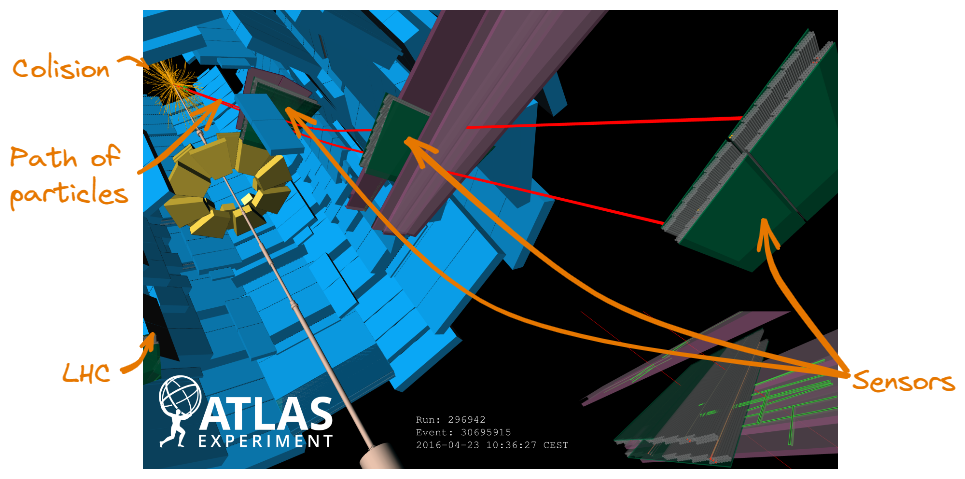
\includegraphics[width=0.85\textwidth]{05-resources/img/spec/experiment-atlas.excalidraw.png}
    \caption{ATLAS experiment at CERN~\cite{atlas-experiment}}
    \label{fig:introduction:particles:tracking}
\end{figure}

\section{Lawrence Berkeley National Laboratory}
\label{ch:introduction:lbl}

The \acrfull{lbl} is a national laboratory in Berkeley, California.
It is managed and operated by the University of California for the \acrfull{doe}.
The lab is situated in the hills of Berkeley and it is composed of many buildings
and has a beautiful view of the San Francisco Bay (see Fig.\ref{fig:introduction:lbl:view}).
This laboratory is mentioned in the recently released movie by Christopher Nolan,
"Oppenheimer".

\begin{figure}[ht]
    \centering
    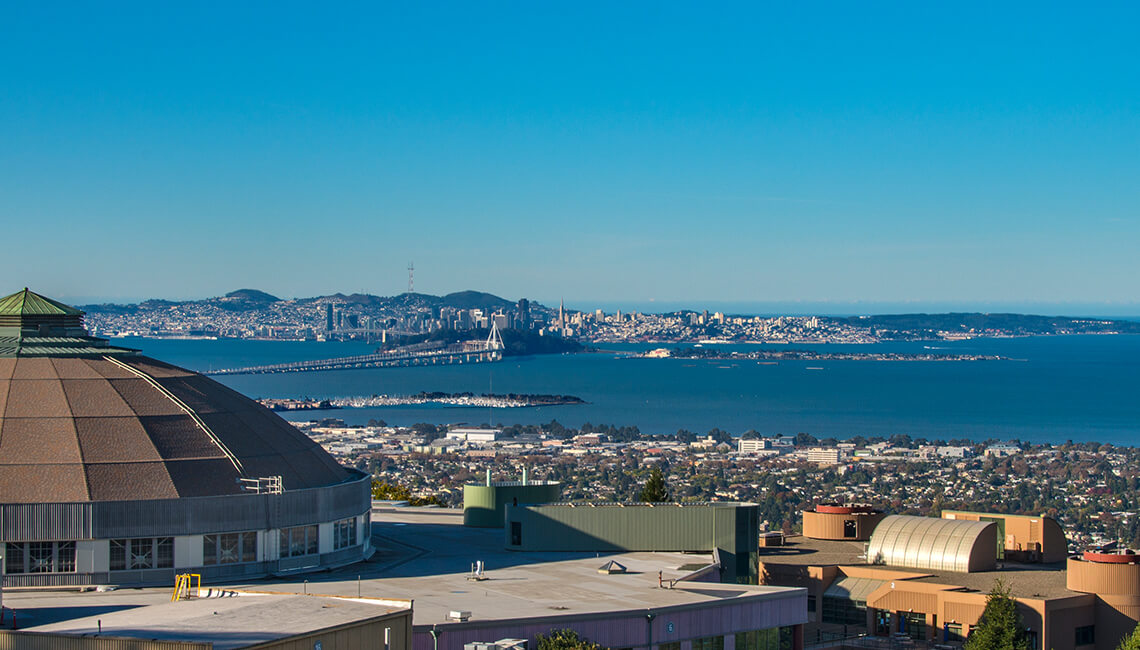
\includegraphics[width=0.8\textwidth]{05-resources/img/spec/lab-view.jpg}
    \caption{Lawrence Berkeley National Laboratory}
    \label{fig:introduction:lbl:view}
\end{figure}


\section{The objectives}
\label{ch:introduction:objectives}

Celeritas is already accelerated by \acrshort{gpu}s, however, the team wants to
improve the performance.
In the current version of the code, each particle track is processed in parallel
by one GPU thread, with no collaboration between threads.
GPU profiling of the code shows that execution time is dominated by two kernels.
The first one is handled by the interaction with the detector geometry to know
where, in 3D space, the particle is situated and during the profiling, the
library used is vecGeom~\cite{VecGeom}.
The second kernel, which will be the focus of this Bachelor thesis project, is
the computation of a differential equation using Dormand-Prince~\cite{princeDormand}.

However, the thesis can be a success even if the project doesn't meet the improvement.
This is because we don't yet know whether thread synchronization will be more
time-consuming than the original version.
In addition, the kernel launch in Celeritas have to be changed, and this
could take up a considerable amount of optimization time.
For the Bachelor thesis, it is sufficient to have a proof of concept that
demonstrates if the enhancement is effective and deserves to be integrated.
To measure the changes done during the internship, the profiler must be run
before and after each step of the project.
The mandatory requirements are described in the following section.

\subsection{Learn GPU programming}
\label{ch:introduction:objectives:learn-gpu-programming}

Before starting to work on the project, some things need to be learned and the goal here is to learn a new way of programming.
To conclude this goal, no code will be produced except for exercises, but the important notions of \acrshort{gpu} programming with CUDA will be synthesized using cheat sheets.
To take advantage of the delay between the beginning of the Bachelor thesis and the beginning of the \acrshort{lbl} internship, this step will be done during this time.


\subsection{Understand the project}
\label{ch:introduction:objectives:understand-the-project}

To be able to improve the performance of the code, the first step is to understand the project and it's always better to understand the background: why it is needed, who will use it and which paradigm and tools are used.

To measure the performance gained, it is necessary to know where the project is at each step.
To take a snapshot of the performance, a profiler can be run and this includes that we can compile and launch the project.
This step will be done at the beginning of the project on-site.


\subsection{Improve the performance}
\label{ch:introduction:objectives:improve-the-performance}

The main goal of the project is to improve the performance of the implementation of Dormand-Prince method~\cite{princeDormand}.
This last mandatory requirement is the core of the thesis and the most important part of the project and it will require the knowledge gained in the first two steps to improve the performance.

To conclude this step, the code must compile, pass the unit test, and a profiler must be run to show the difference between the new and the legacy implementation of the DormandPrince method.
To achieve this goal, the profiles must show an improvement, but this could meet some difficulties to be realized and integrated into the project.
In all cases, the failure of this goal doesn't mean the failure of the thesis if the documentation is correctly done and explains the results obtained and how is it possible or not to continue to this path.
This step will be done after the first two steps and it will take the whole time left.

\section{Optional requirements}
\label{ch:introduction:optional-requirements}

These optional goals are good additions to the project but they are not
require to have a concrete result.

The first one is to have a portable performance.
The purpose of Celeritas is to be run on all kinds of \acrshort{gpu} and even on machines with just a \acrshort{cpu}.
During the optimization, the improvement will be checked on the Perlmutter~\cite{Perlmutter} which uses Nvidia A100 with the architecture Ampere~\cite{ampere} and some improvement can be only effective to this kind of \acrshort{gpu}.
This goal is here to check if the improvement has a positive effect on other architectures and if it is not, to find a way to do that.
To begin this step, the main goal needs to be finished.

The second optional objective is to do another performance improvement.
If the performance of the Runge-Kutta method~\cite{Runge-Kutta-methods} is improved, another optimization can be done.
This part goal will be discussed further in the project with the supervisors and the customers and it will be managed like the last mandatory goal.
This step can be done multiple times if there is enough time.

\chapter{Analysis}
\label{ch:analysis}
% -----------------------------------------------------------------------------
This project starts with a lot of points to analyze.
From the hardware to the technology used, everything has to be analyzed to be able to make a good project.


\section{Microdispenser $\mu$BoMa}
\label{sec:microdispenser}
% -----------------------------------------------------------------------------
\acrshort{dec} has already done a prototype of the microdispenser $\mu$BoMa but the connected part is missing.
The figure~\ref{fig:analysis:microdispenser:protype} shows the prototype of the microdispenser.

\begin{figure}[ht]
    \centering
    
\includegraphics[width=0.4\textwidth]{img/logo}
    \caption{$\mu$BoMa illustration}
    \label{fig:analysis:microdispenser:protype}\end{figure}

Currently, the dispenser must be connected to an industrial computer using several cables to function.
The goal is to replace all the cables and the industrial computer by a microcontroller that will be connected to the dispenser and provide an interface to control it.


\subsection{Electrical interface}
\label{subsec:interface}
the dispenser has the following pins to be managed.
The figure~\ref{fig:analysis:communication:illustration} shows the type of interface used for each device.

\subsubsection{Rotary valve}
\label{subsubsec:serial}
the dispenser has a rotary valve that can open or close the outputs of the tank.
This valve is actioned by a stepper motor that is controlled by a serial interface.
The standard RS-232~\cite{rs-232} defines the electrical characteristics and timing of the signals but not the protocol used.
This protocol is defined by \acrshort{dec} and more information about can be found in the annexes.

\subsubsection{Pressure sensor}
\label{subsubsec:analog}
To manage the pressure, the microdispenser has a pressure sensor and a regulator.
These two devices are connected to the microdispenser with an analog interface.
These interfaces are using the intensity from 4 to 20mA~\cite{analog} to control the pressure and the volts from 1 to 5~V to read the information.
If the values don't start at 0, it's to detect if the device is connected or not.

\subsubsection{Bubble's detector}
\label{subsubsec:digital}
To detect if there is some bubbles in the tank, the microdispenser has a digital pin.
Now, the tank doesn't have any bubble detector but the sensor still exists anyway.


\section{Communication}
\label{sec:communication}
% -----------------------------------------------------------------------------

To summarize, the microcontroller must be able to communicate with the microdispenser through the electrical interface and with the user.
The figure~\ref{fig:analysis:communication:illustration} shows all the communication medium.

\begin{figure}[ht]
    \centering
    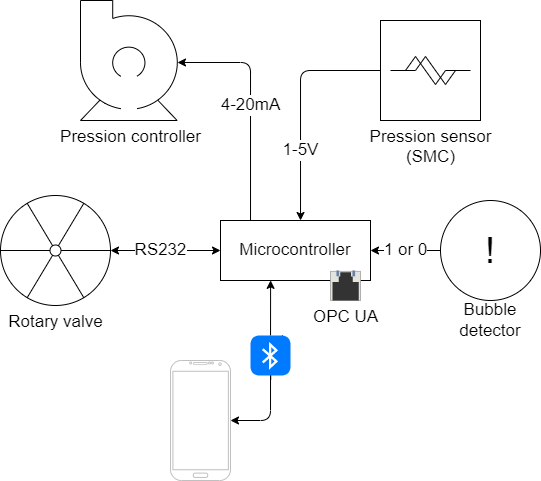
\includegraphics[width=0.8\textwidth]{img/communication.drawio}
    \caption{Communication illustration}
    \label{fig:analysis:communication:illustration}
\end{figure}

The \acrshort{mvp} can be used in different environments and the communication medium must be adapted to each of them.

\subsection{Laboratory}
\label{subsec:laboratory}
In the laboratory environment, the $\mu$BoMa works in standalone.
To order a dispense, the user must use a client application to communicate with the microcontroller.

\subsubsection{Client application}
\label{subsubsec:client}
The client application is a mobile application that uses the Bluetooth to communicate with the microcontroller.
This application is very simple and it only has a text field to enter the volume to dispense and a button to send the order.
The figure~\ref{fig:analysis:communication:laboratory:client} shows the sketch of the application.

\begin{figure}[ht]
    \centering
    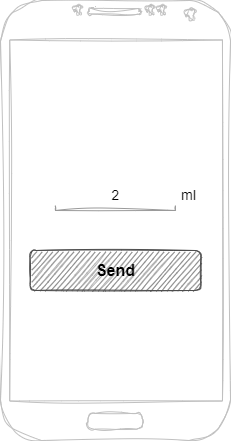
\includegraphics[width=0.3\textwidth]{img/mobapp_sketch.drawio}
    \caption{Client application Illustration}
    \label{fig:analysis:communication:laboratory:client}
\end{figure}

This application is developed with the framework Flutter~\cite{flutter}.
This framework is a cross-platform framework that allows them to develop an application for Android, iOS and web using the code Dart.
It's initially developed by Google and now it's open source.

\subsubsection{Bluetooth}
\label{subsubsec:bluetooth}
The Bluetooth is a wireless technology that allows them to communicate between two devices.
It's a low-power technology that is used in a lot of devices like smartphones, smartwatch and now even more in the laptop.

\subsection{Production}
\label{subsec:ethernet}
When the microdispenser will be used in production, the communication and the power supply will be done with \acrfull{poe}.
This technology allows us to transmit data and power over a single cable.

\subsubsection{OPC UA}
\label{subsubsec:opc}
The communication between the microcontroller and the industrial computer will be done with the \acrfull{opc}~\cite{opc} protocol.
This is a machine-to-machine secure and reliable protocol there is widely used in the industry.
It's a standard protocol oriented service designed to provide a platform-independent.

There is a library for C++~\cite{open62541_2023} that implements \acrshort{opc}.

\section{Microcontroller}
\label{sec:mcu}
% -----------------------------------------------------------------------------
The microcontroller will be the heart of the project.
The chosen one must meet the requirements of the project.
That includes the pins available, the speed, the memory, the availability on the market and the module that can be added to it.
\acrshort{dec} Provide high quality solutions so a top microcontroller can be chosen.

\newpage
\subsection{Requirements}
\label{subsec:requirements}
The table~\ref{tab:analysis:mcu:criteria} is the requirements that the microcontroller must meet to be chosen.
If one of the mandatory cannot be met, the microcontroller will automatically be rejected.

The mandatory criteria required are those where the value is to `Yes'.
In the other case, the number between 0 and 5 shows the relevant of these criteria and this coefficient will be used to compute the score of each microcontroller.


\begin{table}[ht]
    \centering
    \begin{tabular}{|p{2.6cm}|p{2cm}|p{8cm}|}
    \hline
    \multicolumn{1}{|c|}{\textbf{Criteria}} &
      \textbf{Mandatory or Relevant} &
      \multicolumn{1}{c|}{\textbf{Description}} \\ \hline
      \textbf{4-20mA pin}                  & Yes & this pin is to control the pressure in the tank \\ \hline
      \textbf{1-5V pin}                    & Yes & This pin is used to read the pressure from the sensor \\ \hline
      \textbf{Bluetooth/WiFi module}       & Yes & This requirement is needed for the laboratory environment \\ \hline
      \textbf{Ethernet interface}          & Yes & \acrshort{dec} wants to connect their device with a cable due to the stability in a production line \\ \hline
      \textbf{\acrshort{opc}}              & Yes & In the production line environment, the dispenser will communicate with the protocol \acrshort{opc} and the microcontroller must be compatible \\ \hline
      \textbf{Availability on the market} & 5 & It's one of the most important criteria of microcontroller the last years.\\ \hline
      \textbf{Development support}         & 4 & The development provided can be very useful to be productive \\ \hline
      \textbf{Processing power}            & 3 & The microcontroller will probably manage more than one thread at the time \\ \hline
      \textbf{Memory}                      & 2 & Until the program can run without memory errors, this point isn't relevant because the data won't be stored locally \\ \hline
      \textbf{\acrshort{poe}}              & 2 & \acrfull{poe} could be nice to have a cleaner installation. \\ \hline
      \textbf{Learning curve}              & 2 & To accelerate the project, it could be nice if the microcontroller is known \\ \hline
      \textbf{Cost}                        & 1 & \acrshort{dec} would prioritize the quality over the cost \\ \hline
    \textbf{Autonomy} &
      0 &
      The power consumption isn't relevant in this case because the microdispenser will always be connected to something \\ \hline
    \end{tabular}
    \caption{Criteria for the microcontroller}
    \label{tab:analysis:mcu:criteria}
\end{table}

\subsection{Candidates}
\label{subsec:candidates}
The following microcontroller are candidates for the project.
The candidates will be judged with the criteria of the table~\ref{tab:analysis:mcu:criteria}.

\subsubsection{Raspberry pi}
\label{subsubsec:mcu:candidates:pi}
They are a very popular series of single-board computers.
Actually, there is a multiple version and it can be used with Linux distribution.

The Raspberry Pi 4 Model B is the most recent and powerful version~\cite{pi4}.
It's a quad core 64-bit ARM Cortex-A72 processor running at 1.5~GHz and the memory can be 2~GB, 4~GB or 8~GB\@.
This board provides an Ethernet interface, a Bluetooth module and a serial interface.
It's also possible to add an extension to use the 4--20mA pins~\cite{ncdio_2022}.


\subsubsection{STM32}
\label{subsubsec:mcu:candidates:stm32}
STM32 is a series of microcontroller from STMicroelectronics.
There is a multiple version of this microcontroller and it's possible to add an ethernet module and a Bluetooth module.
There are some versions that have a cortex A core, which they are compatible with a Linux this simplifies the usage of the library~\cite{open62541_2023} for the \acrshort{opc}.

\subsubsection{ESP32}
\label{subsubsec:mcu:candidates:esp32}
This is a very popular microcontroller in the \acrfull{iot} world.
It's a dual core 32-bit microcontroller with a clock speed of 240~MHz.
He adds a Bluetooth module and a wifi module and it's also possible to add an ethernet module.
The ESP32 uses a \acrfull{rtos}~\cite{rtos_2023}.

\subsubsection{Arduino}
\label{subsubsec:mcu:candidates:arduino}
Arduino provide microcontrollers and development boards.
The Arduino Uno is the most popular and it's a microcontroller with an 8-bit AVR microcontroller at 16~MHz.
It's possible to add an ethernet shield to use the Ethernet interface and a Bluetooth module.
Arduino use a \acrfull{rtos}~\cite{rtos_2023}.

\newpage
\subsection{Choice}
\label{subsec:choice}
To choice the best microcontroller, the multi-criterion matrix from the table~\ref{tab:analysis:mcu:criteria} will be used.

\begin{table}[ht]
  \centering
  \begin{tabular}{|p{2.6cm}|p{2cm}|c|c|c|c|}
  \hline
  \multicolumn{1}{|c|}{\textbf{Criteria}} &
    \textbf{Mandatory or Relevant} &
    \textbf{Pi} &
    \textbf{STM32} &
    \textbf{ESP32} &
    \textbf{Arduino} \\ \hline
    \textbf{4-20mA pin}                  & Yes & Yes & Yes & Yes & Yes \\ \hline
    \textbf{1-5V pin}                    & Yes & Yes & Yes & Yes & Yes \\ \hline
    \textbf{Bluetooth/WiFi module}       & Yes & Yes & Yes & Yes & Yes \\ \hline
    \textbf{Ethernet interface}          & Yes & Yes & Yes & Yes & Yes \\ \hline
    \textbf{\acrshort{opc}}              & Yes & Yes & Yes & \textbf{No} & \textbf{No} \\ \hline
    \textbf{Availability on the market}  & 5 &   1 & 1 & - & - \\ \hline
    \textbf{Development support}         & 4 &   3 & 2 & - & - \\ \hline
    \textbf{Processing power}            & 3 &   3 & 2 & - & - \\ \hline
    \textbf{Memory}                      & 2 &   3 & 2 & - & - \\ \hline
    \textbf{\acrshort{poe}}              & 2 &   2 & 3 & - & - \\ \hline
    \textbf{Learning curve}              & 2 &   3 & 2 & - & - \\ \hline
    \textbf{Cost}                        & 1 &   1 & 2 & - & - \\ \hline
  \multicolumn{2}{|l|}{\textbf{Total}}    & \textbf{43} & 37 & - & - \\ \hline
  \end{tabular}
  \caption{Choice of the microcontroller}
  \label{tab:analysis:mcu:choice}
\end{table}

The \acrshort{opc} library~\cite{open62541_2023} requires a Linux distribution and only the Pi and the STM32 can be used with a Linux kernel.
There is some work in progress to adapt the library to the \acrshort{rtos} but it's not stable yet.
The Raspberry Pi is better while it offers a better development platform and he can be more adaptable with the different modules.
To reduce the size in a production environment, with can use a NanoPi or a PiCompute.

\subsection{Raspberry PI}
\label{subsec:pi}
To do the \acrshort{mvp}, the simple way is to use a Raspberry Pi 4 Model B\@.
These boards are very popular and they are easy to use.
The figure~\ref{fig:analysis:mcu:pi} shows the Raspberry Pi 4 Model B\@.

\begin{figure}[ht]
  \centering
  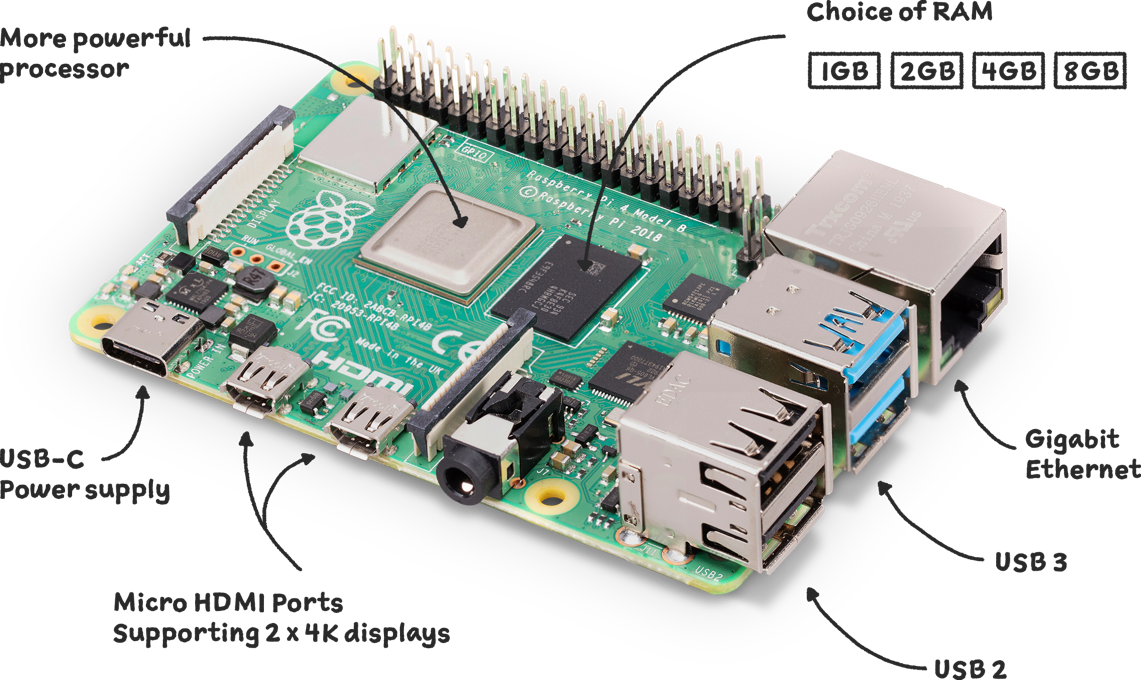
\includegraphics[width=0.6\textwidth]{img/raspberry-pi-4}
  \caption{Raspberry Pi 4 Model B~\cite{raspberryPi4}}
  \label{fig:analysis:mcu:pi}
\end{figure}

To bring on\acrshort{mvp} a production environment, we can use a NanoPi or a PiCompute.
These boards are smaller and they can be more adapted to a production environment.
The advantage of the PiCompute is that it's possible to develop a custom board with the same footprint.
As they are the same processors, the code developed on one can be ported to another.


\subsection{Clickboard}
\label{subsec:clickboard}

Mikroe provides modules named Clickboard~\cite{mikroe-shield}.
These modules are easy to use while they can be plugged on a shield.

\begin{figure}[ht]
  \centering
  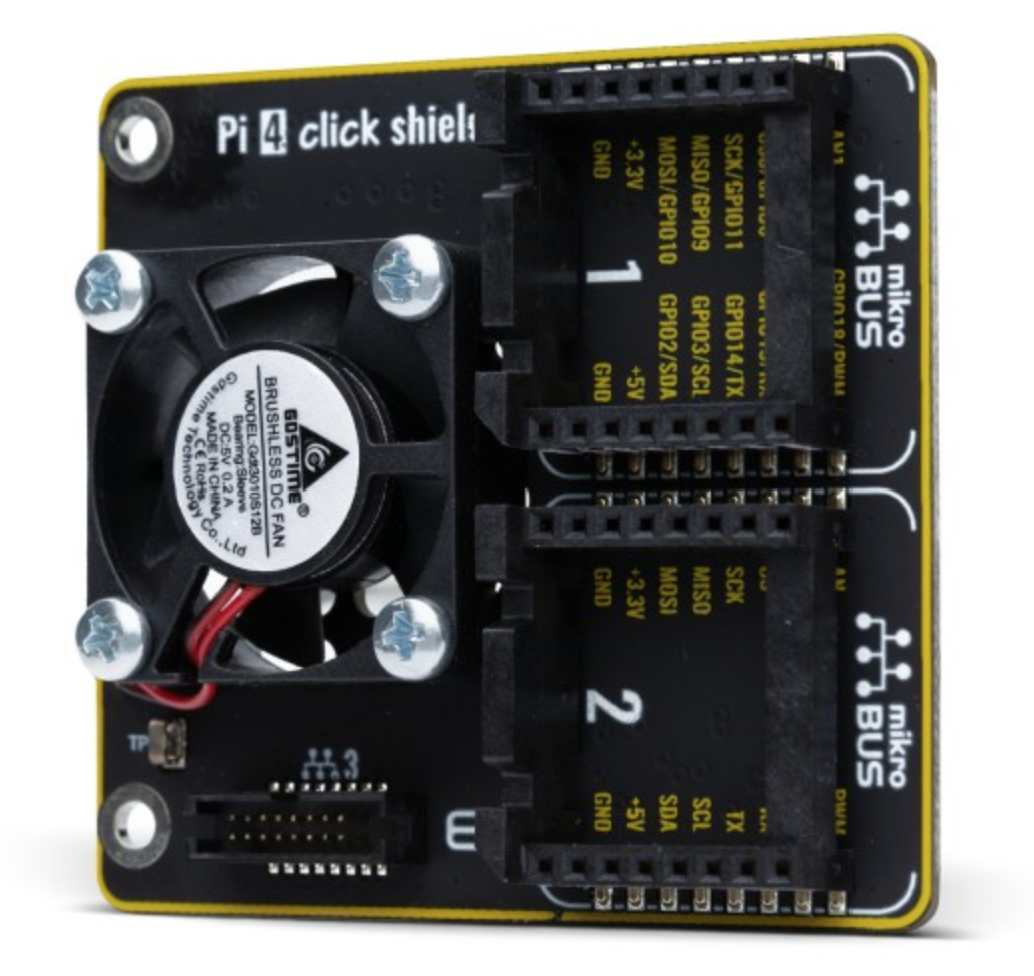
\includegraphics[width=0.4\textwidth]{img/mikroe-shield}
  \caption{Clickboard~\cite{mikroe-shield}}
  \label{fig:analysis:mcu:clickboard}
\end{figure}

The shield on the figure~\ref{fig:analysis:mcu:clickboard} can be plugged on a Raspberry Pi 4 and it has 2 mikroBus slots directly on the board and one that can be plugged with an extension cable.


\subsubsection{RS232}
\label{subsubsec:rs232}
To communicate with the standard RS232~\cite{rs-232}, it's possible to use a USB to RS232 converter but it's not the best solution.
If the final board is a custom board, it's possible there is no USB port.
To avoid this problem, it's possible to use a RS232 clickboard interface.
The figure~\ref{fig:analysis:mcu:rs232} shows this module.

\begin{figure}[ht]
  \centering
  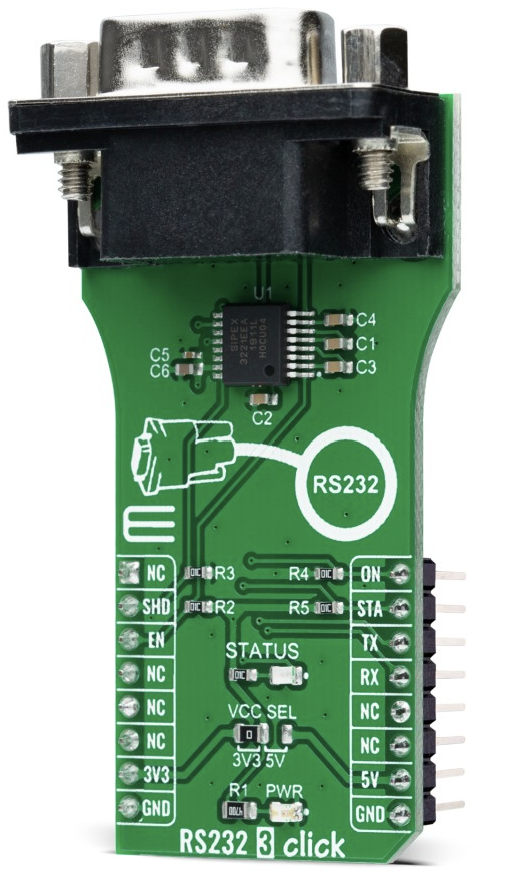
\includegraphics[width=0.15\textwidth]{img/rs232-converter}
  \caption{RS232 to Raspberry Pi~\cite{mikroe-rs232}}
  \label{fig:analysis:mcu:rs232}
\end{figure}

It would be plugged on the clikcboard shield.

\subsubsection{4-20mA}
\label{subsubsec:4-20ma}
To control the pressure in the tank, the microcontroller must provide an intensity between 4 and 20 mA\@.
However, the Raspberry Pi doesn't have this feature, there is a click board that can be used.
The figure~\ref{fig:analysis:mcu:4-20mA} shows this click board that is controlled by the Raspberry Pi through the SPI interface.

\begin{figure}[ht]
  \centering
  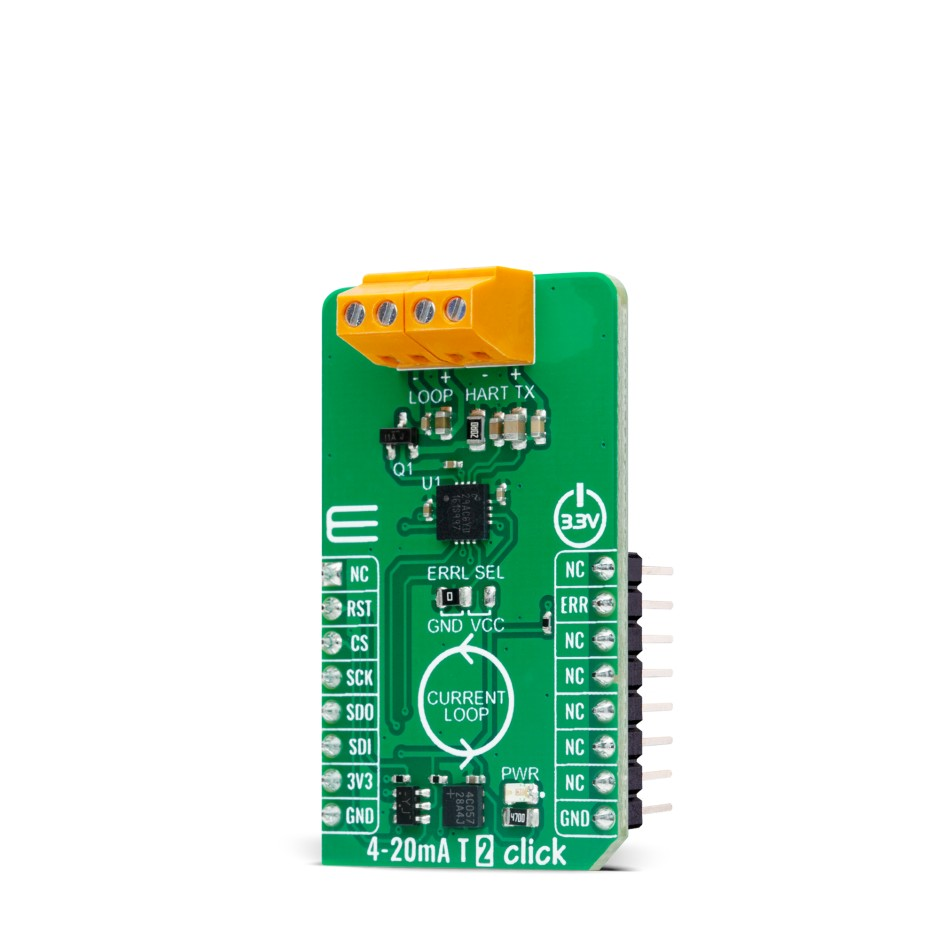
\includegraphics[width=0.3\textwidth]{img/4-20ma}
  \caption{4-20mA T 2 click~\cite{mikroe-420ma}}
  \label{fig:analysis:mcu:4-20mA}
\end{figure}

\subsubsection{1-5V}
\label{subsubsec:1-5v}
To read the pressure in the tank, the microcontroller must read a voltage between 1 and 5~V\@.
Like the 4--20mA, the Raspberry Pi doesn't have this feature and a module is required.
The figure~\ref{fig:analysis:mcu:1-5V} shows a board that can be added to the clickboard shield and controlled by the Raspberry Pi through the SPI interface.

\begin{figure}[ht]
  \centering
  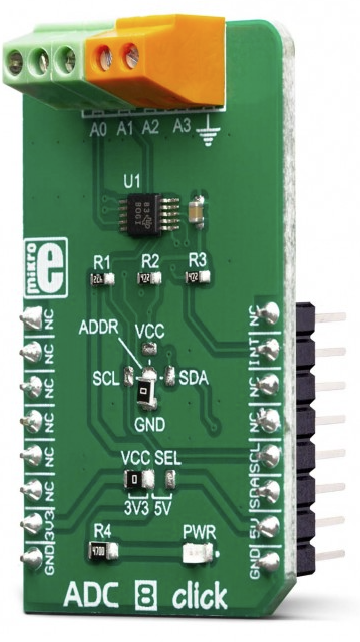
\includegraphics[width=0.15\textwidth]{img/raspberry-1_5V}
  \caption{ADC 1--5V~\cite{mikroe-15v}}
  \label{fig:analysis:mcu:1-5V}
\end{figure}


\subsection{PoE}
\label{subsec:poe}
There is a \acrshort{poe} hat for the Raspberry Pi 4 Model B and the Raspberry Pi 3 Model B/B+.
however, this module isn't relevant for the \acrshort{mvp} but it's interesting for the production environment.
The figure~\ref{fig:analysis:mcu:poe} shows the hat on the Raspberry Pi 4 Model B\@.

\begin{figure}[ht]
  \centering
  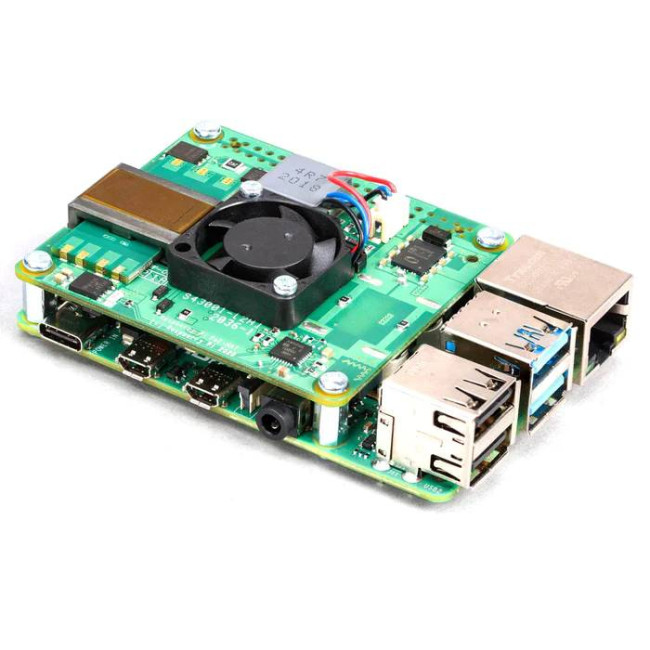
\includegraphics[width=0.3\textwidth]{img/raspberry-poe}
  \caption{PoE HAT~\cite{pi-shop}}
  \label{fig:analysis:mcu:poe}
\end{figure}
\section{Programming language}
\label{sec:lang}
% -----------------------------------------------------------------------------
The programming language is the main tool to produce the \acrshort{mvp}.
It must be chosen carefully because it will be used for the whole project.
To be selected, the language must be able to control the pin of the microcontroller and to communicate with the \acrshort{opc} server.

\subsection{Tiny GO}
\label{subsec:go}
Tiny GO~\cite{tinygo} is a compiler for the language GO~\cite{go} that as for purpose to compile for microcontroller.
Go (aka Golang) is a language created by Google in 2007 and it's now open source.
The purpose is to improve productivity and fit to the multicore networked machines of today.
This language is compiled and statically typed that make it fast and lightweight.
The dependency management and the formatter are built-in that increase the robustness of the project.

\subsection{C}
\label{subsec:c}
C is a language created in 1972.
It's compiled and statically typed and it's very fast.
It's used in many projects and it was very popular until the oriented object language appeared.
Actually, this language is still used in many projects but it isn't easy to learn and it has lack of features like the garbage collector.


\subsection{C++}
\label{subsec:cpp}
C++ is an old object-oriented language created in 1983.
Like GO, it's compiled and statically typed but there is no garbage collector.
The language is very powerful and it's used in many projects.
There is a huge community behind C++ and the embedded programming and the libraries are offently written in C++ and it allows to use C library.

\subsection{MicroPython}
\label{subsec:micropython}
MicroPython~\cite{micropython} is a python implementation for microcontroller.
Python is a high-level language created in 1991.
It's interpreted and dynamically typed and it's very easy to learn.
The language is very popular and there is a lot of libraries available.
This implementation is optimized for microcontroller and it's possible to use it on the Raspberry Pi and many other microcontrollers.

\subsection{Conclusion}
\label{subsec:conclusion}
To complete this case, the best language is C++ because it's the most used language in the embedded world.
The \acrshort{opc} library~\cite{open62541_2023} is written in C++ and there is a variant in other language but the C++ version is the most complete.
\acrshort{dec} They are also using C++ in their project and it's a good point to have a common language.



\section{Development environment}
\label{sec:dev}
% -----------------------------------------------------------------------------
To develop the \acrshort{mvp}, it's necessary to have a development environment.

\subsection{IDE}
\label{subsec:ide}
During the project, the IDE from jetbrains are used.
For the core part, the IDE is CLion and for the client part, that IntelliJ with the Flutter plugin.
To develop directly on the Raspberry Pi from a computer, it's possible to create a Cmake profile that uses a toolchain that is connected to the Raspberry Pi through SSH.

\begin{figure}[ht]
  \centering
  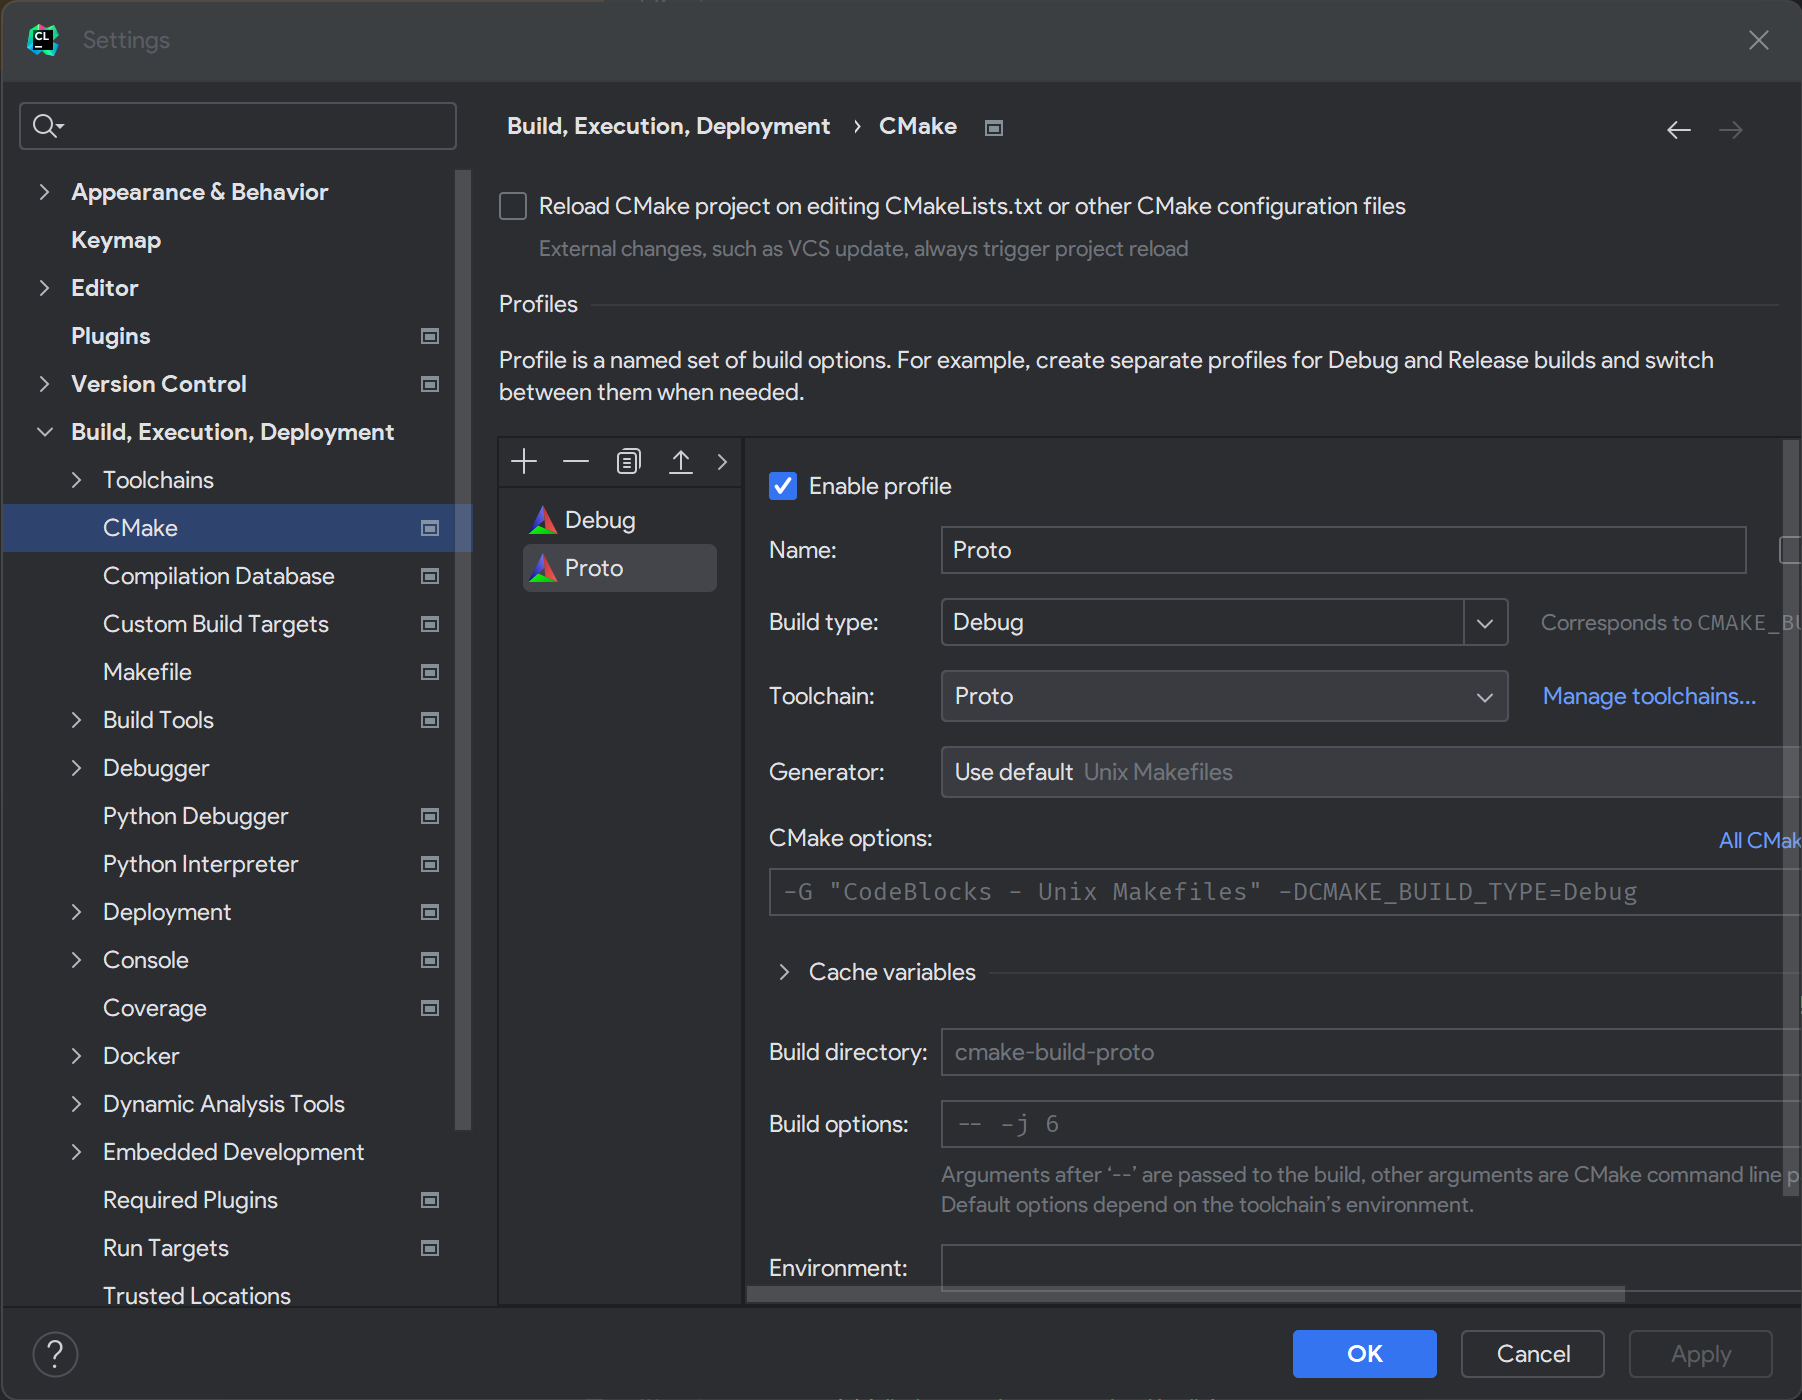
\includegraphics[width=0.75\textwidth]{img/analyze_cmake-profile.png}
  \caption{CMake profile on CLion}
  \label{fig:analysis:dev:clion}
\end{figure}

In the figure~\ref{fig:analysis:dev:clion}, it's possible to see the CMake profile that is used to compile the code on the Raspberry Pi.
The toolchain Proto is a toolchain defined in the Clion settings that is connected to the Raspberry Pi through SSH.

\subsection{Pre-commit}
\label{subsec:pre-commit}

It's recommended to use a pre-commit tool to check the code before committing it.

To install this tool on the computer, it's necessary to have python and install the packages that are mentioned in the file \texttt{requirements-dev.txt}.
Then, to install the hook script, it just needs to run the command \texttt{pre-commit install}.
All these files are at the root of the project.

The following figure \ref{fig:analysis:dev:pre-commit} show what's happened when a git commit is done.

\begin{figure}[ht]
  \centering
  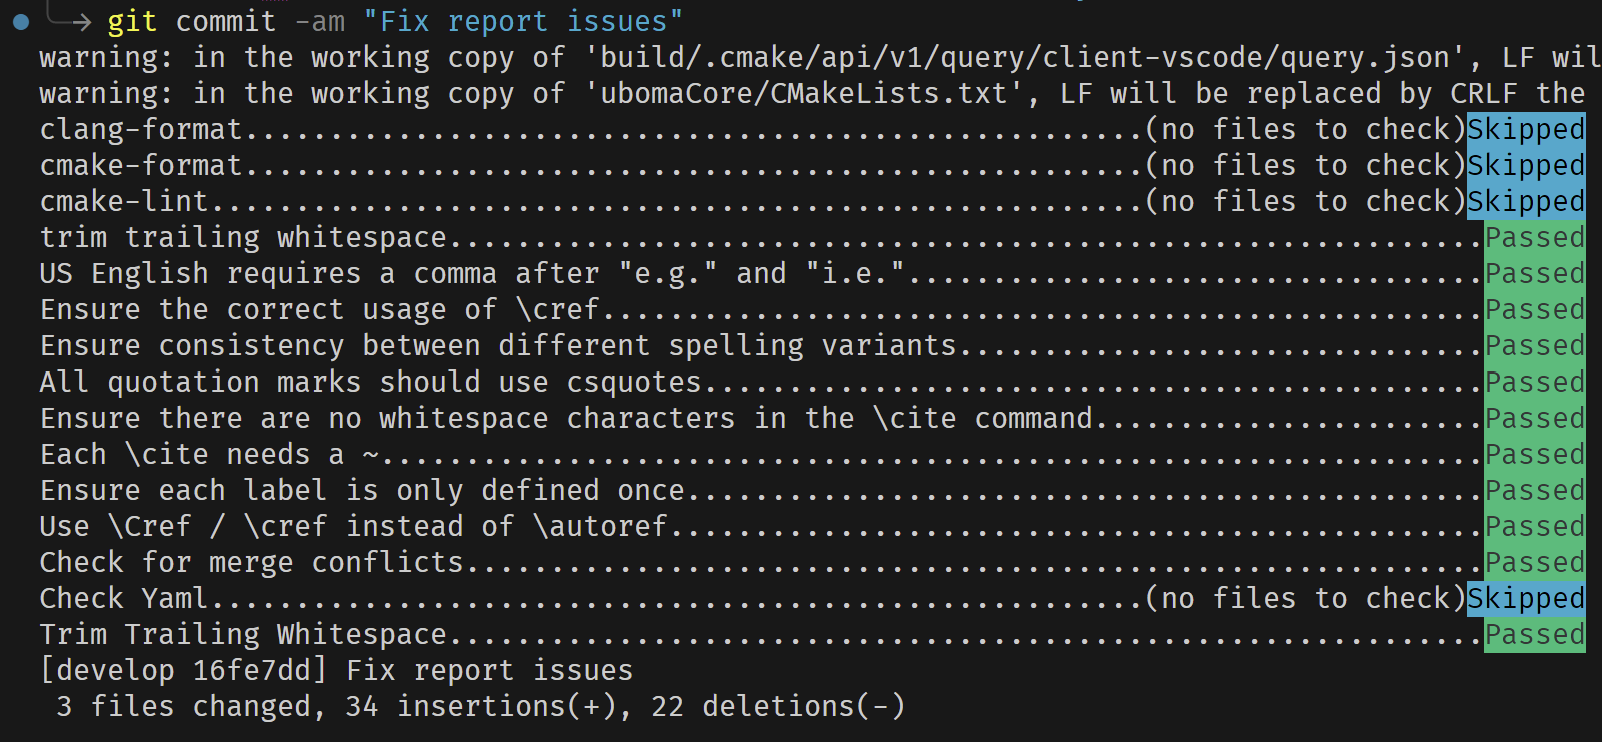
\includegraphics[width=0.75\textwidth]{img/analyze_pre-commit.png}
  \caption{Pre-commit}
  \label{fig:analysis:dev:pre-commit}
\end{figure}


\chapter{Conception}
\label{ch:conception}

All the components of the system or how they are connected to each other are described in this chapter.
The map of the pins is also described in this chapter.

% ---------------------------------------------------------
\section{Core application}
\label{conception:core-application}

The core application is the application that is installed on the Raspberry Pi and she's responsible for the communication with the devices and the clients.
This application is written in C++ and uses the WiringPi library to communicate with the devices and REST API with web sockets to communicate with the clients.

\subsection{Packages}
\label{conception:core-application:packages}

The core application is divided into two parts.

The first part is the communication with the devices.
This part is to simplify the usage of the devices and hide the complexity of the communication.
This part uses the WiringPi library to communicate with the devices.

The second part is the communication with the clients.
This part is the REST API and the web socket.
The REST API is used to configure the devices and the web socket is used to send the data to the clients.
He uses the first part to communicate with the devices.

There is also a third part that is a singleton that stores the state of the application.
This part is used by the device’s part to store the information and by the REST API to send the information to the clients.

\begin{figure}[ht]
  \centering
  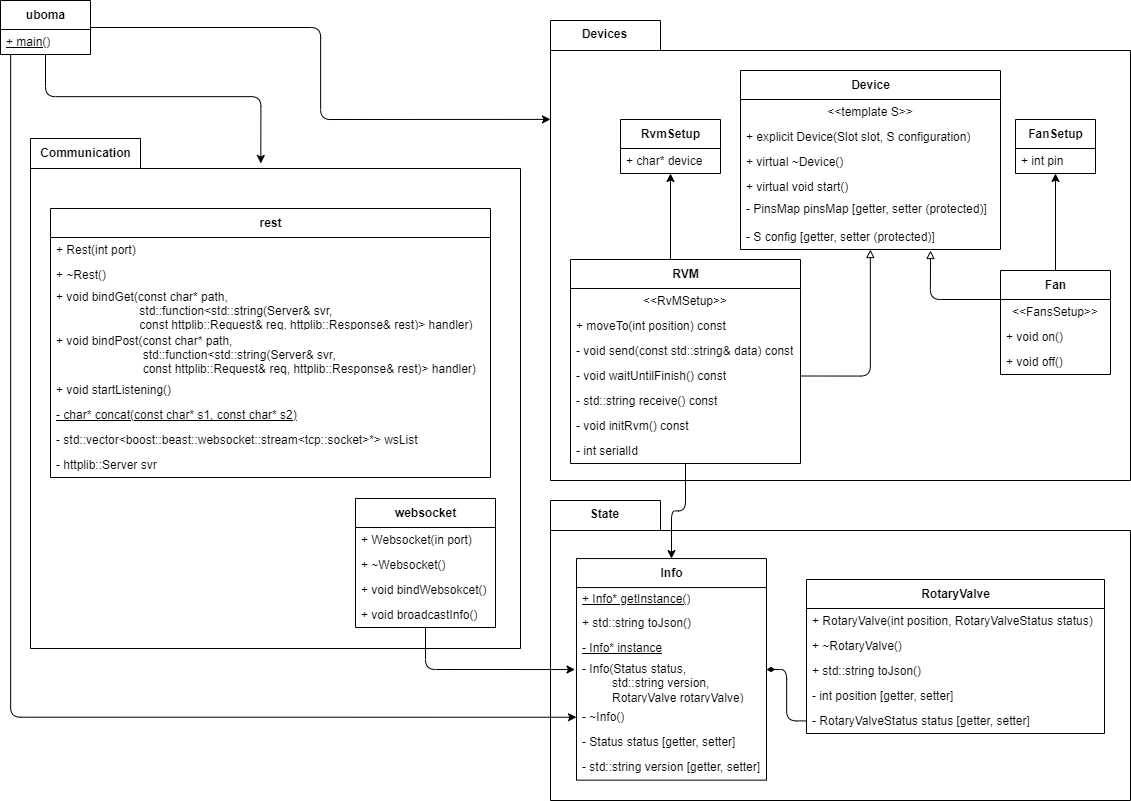
\includegraphics[width=1\textwidth]{img/conception_packages.drawio.png}
  \caption{Core application packages}
  \label{fig:conception:core-application:packages:illustration}
\end{figure}

The figure \ref{fig:conception:coreApplication:packages:illustration} illustrate the packages of the core application.
There is no link between the communication and the devices because the action of the route of the REST API are directly defined in the uboma.

\subsection{Threads}
\label{conception:core-application:threads}

The core application must manage many tasks at the same time, so it uses threads to do that.
The main thread starts to initialize all the devices and the route of the REST API.
The handling of the REST API is done in a thread that will create a new thread for each request.
The main thread will also listen to the web socket and create a new thread for each new client.
The figure \ref{fig:conception:coreApplication:threads:illustration} illustrate the relation of each thread.

\begin{figure}[ht]
  \centering
  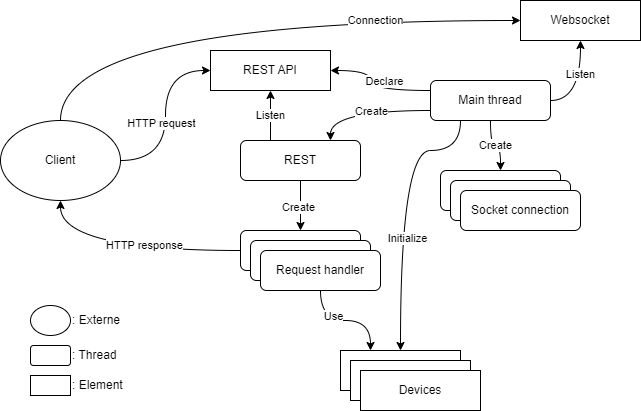
\includegraphics[width=1\textwidth]{img/conception_threads.drawio.png}
  \caption{Threads illustration}
  \label{fig:conception:core-application:threads:illustration}
\end{figure}

\subsection{Register routes}
\label{conception:core-application:register-routes}
 To register the routes of the REST API, the core application must provide a route and the handler to the class `Rest`.
 This class will set default header to match with the \acrfull{cors} policy and register the route with the handler.

 \begin{figure}[ht]
  \centering
  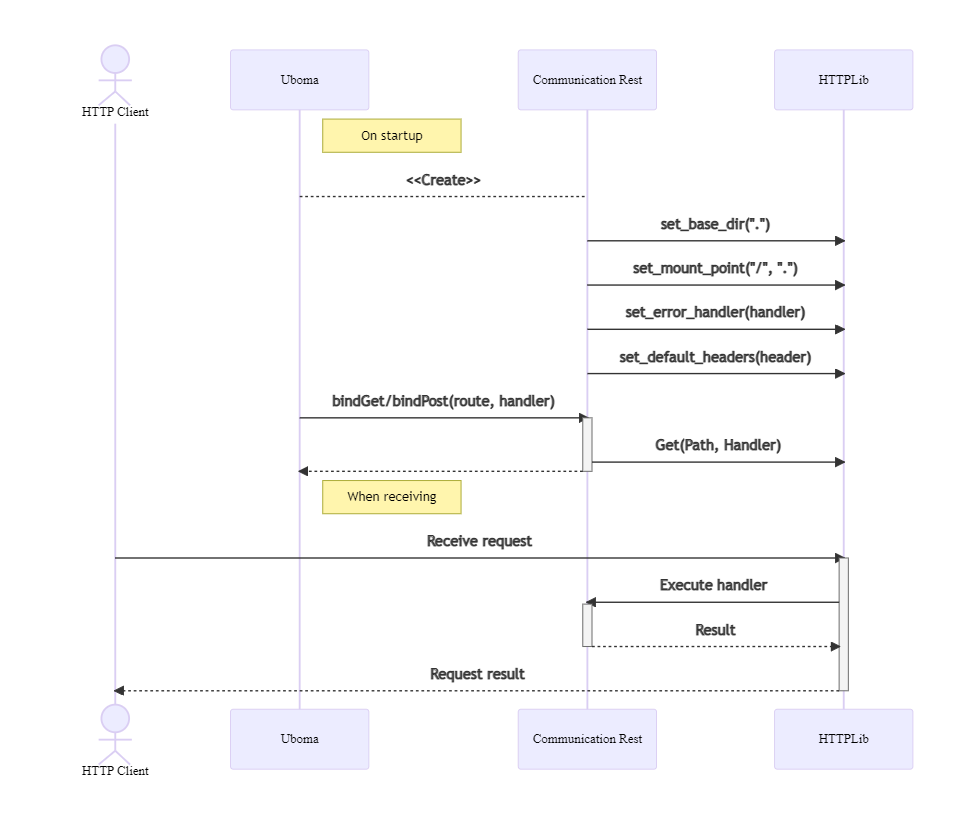
\includegraphics[width=1\textwidth]{img/conception_routes.drawio.png}
  \caption{Register routes sequence}
  \label{fig:conception:core-application:register-routes:illustration}
 \end{figure}

The figure \ref{fig:conception:core-application:register-routes:illustration} illustrate the sequence to register a route and what is made when a request is received.
The class `Rest` surcharge the `HTTPLib` class to add the default header and use thread to listen to the requests.
When a request is received, the class will call the handler.


% ---------------------------------------------------------
\section{Client application}
\label{conception:client-application}

The client application is the application that will be used by the user to interact with the core application.
This application is written in Flutter and use REST API and web socket to communicate with the core application.
Flutter is a framework to create a cross-platform application and it can easily be compiled for Android, iOS, Windows, Linux and MacOS.

\subsection{Mockup}
\label{conception:client-application:mockup}

This is the mockup of the application, the first page of the figure \ref{fig:conception:client-application:mockup:illustration} is the home page.
This page will allow us to do a classic dispense and show the status of the whole system.
The second page is the advanced page.
Each device can be configured and the all his data can be seen.

\begin{figure}[h]
  \centering
  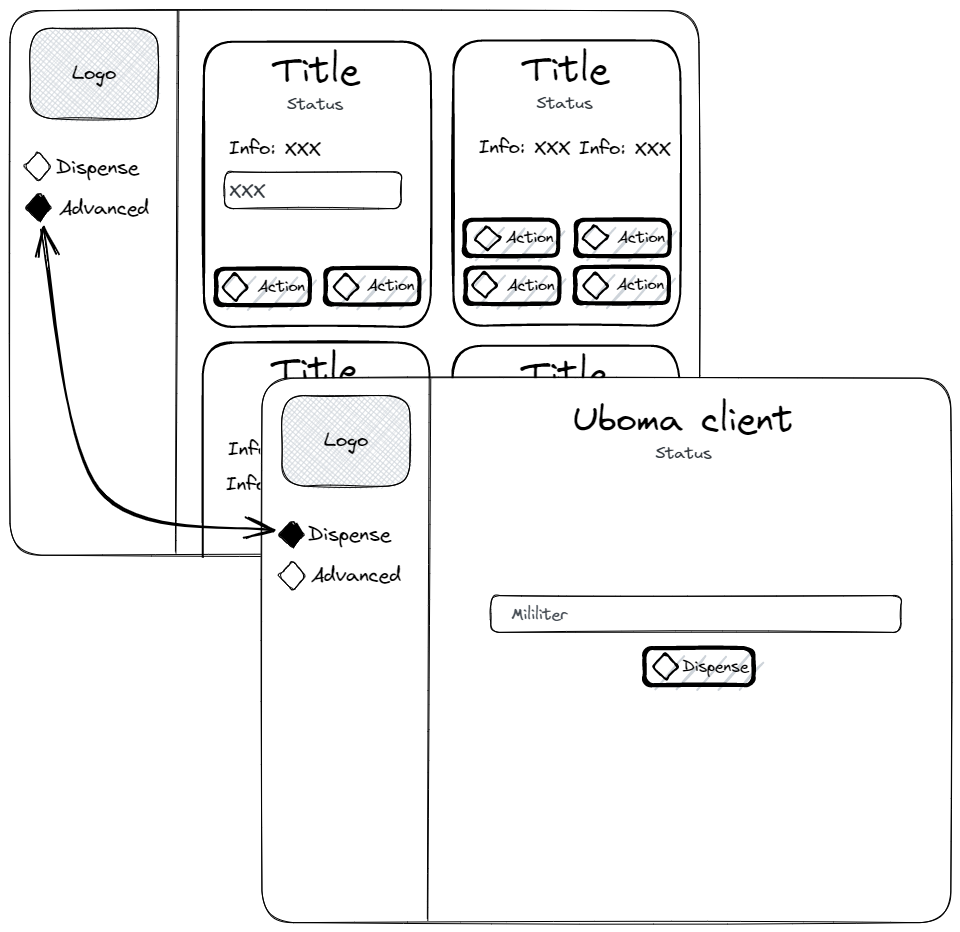
\includegraphics[width=0.65\textwidth]{img/conception_clientApp.excalidraw.png}
  \caption{Mockup of the application}
  \label{fig:conception:client-application:mockup:illustration}
\end{figure}

The cards represent the devices and they will be adapted to each device.

\subsection{Architecture}
\label{conception:client-application:architecture}

The client application follows the \acrfull{mvvm} pattern.
This pattern is used to separate the logic of the application from the view.
The data are managed by a repository which uses the REST API to communicate with the core application.
There \acrshort{mvvm} is a little bit violated because the view is directly linked to the repository.

\begin{figure}[h]
  \centering
  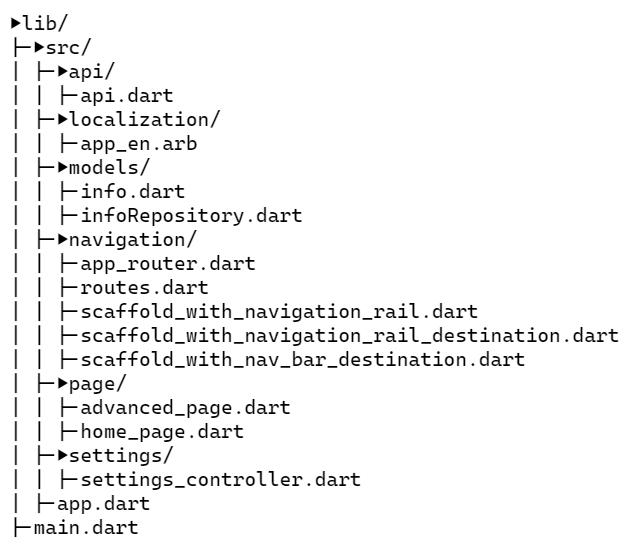
\includegraphics[width=0.55\textwidth]{img/conception_architecture.excalidraw.png}
  \caption{Client application architecture}
  \label{fig:conception:client-application:architecture:illustration}
\end{figure}

The figure \ref{fig:conception:client-application:architecture:illustration} shows the architecture of the client application.
The view is defined in the `page` folder and they are the `Info` stored in the repository.
The files in `localization` are used to translate the application.
To add a new language, a new file must be created in this folder.
The navigation has its own folders and there are multiple files because the application is responsive and the navbar is moving to the bottom on mobile.



\section{Pins}
\label{sec:pins}

The number of the pins of the library WiringPi isn't the same as the number in schema of Mikroe for the shield.
The following table \ref{tab:pin-map} shows the correspondence between the pins of the library WiringPi and the pins of the shield.

% \usepackage{tabularray}
\begin{longtblr}[
    caption = {Pins map},
    label = {tab:pin-map},
  ]{
    row{1} = {c},
    row{2} = {c},
    cell{1}{1} = {r=2}{},
    cell{1}{2} = {r=2}{},
    cell{1}{3} = {r=2}{},
    cell{1}{4} = {r=2}{},
    cell{1}{5} = {c=3}{},
    vline{1-6} = {1-2}{},
    vline{6-8} = {2}{},
    vline{1,8} = {1-41}{},
    hline{1,3-42} = {-}{},
    hline{2} = {5-7}{},
  }
  \textbf{\# } & \textbf{Name } & \textbf{WiringPi } & \textbf{Shield }   & \textbf{Slot } &              &              \\
                     &                &                    &                    & \textbf{One}   & \textbf{Two} & \textbf{Ext} \\
  1                  & 3.3v           &                    &                    &                &              &              \\
  2                  & 5v             &                    &                    &                &              &              \\
  4                  & 5v             &                    &                    &                &              &              \\
  5                  & SCL1           & 9                  & GPIO3/I2C-SCL      & SCL            & SCL          & SCL          \\
  6                  & 0v             &                    &                    &                &              &              \\
  7                  & GPIO7          & 7                  & GPIO4              &                &              &              \\
  8                  & TxD            & 15                 & GPIO14/UART-TX     & TX             & TX           & TX           \\
  9                  & 0v             &                    &                    &                &              &              \\
  10                 & RxD            & 16                 & GPIO15/UART-RX     & RX             & RX           & RX           \\
  11                 & GPIO0          & 0                  & GPIO17             &                &              &              \\
  12                 & GPIO1          & 1                  & GPIO18/PWM1        & PWM            &              &              \\
  13                 & GPIO2          & 2                  & GPIO27             &                &              & INT          \\
  14                 & 0v             &                    &                    &                &              &              \\
  15                 & GPIO3          & 3                  & GPIO22             &                &              & RST          \\
  16                 & GPIO4          & 4                  & GPIO23/CS2         &                &              & CS           \\
  17                 & 3.3v           &                    &                    &                &              &              \\
  18                 & GPIO5          & 5                  & GPIO24             &                &              &              \\
  19                 & MOSI           & 12                 & GPIO10/SPI-MOSI~ ~ & MOSI           & MOSI         & MOSI         \\
  20                 & 0v             &                    &                    &                &              &              \\
  21                 & MISO           & 13                 & GPIO9/SPI-MISO~ ~  & MISO           & MISO         & MISO         \\
  22                 & GPIO6          &                    & SPIO25/DRDY~ ~     &                &              &              \\
  23                 & SCLK           & 14                 & GPIO11/SPI-SCK~ ~  & SCK            & SCK          & SCK          \\
  24                 & CE0            & 10                 & GPIO8/CS0          & CS             &              &              \\
  25                 & 0v             &                    &                    &                &              &              \\
  26                 & CE1            & 11                 & GPIO7/CS1~ ~       &                & CS           &              \\
  27                 & SDA0           & 30                 & -                  &                &              &              \\
  28                 & SCL0           & 31                 & -                  &                &              &              \\
  29                 & GPIO21         & 21                 & GPIO5              & RST            &              &              \\
  30                 & 0v             &                    &                    &                &              &              \\
  31                 & GPIO22         & 22                 & GPIO6~ ~           & INT            &              &              \\
  32                 & GPIO26         & 26                 & GPIO12             &                & RST          &              \\
  33                 & GPIO23         & 23                 & GPIO13/PWM2        &                & PWM          &              \\
  34                 & 0v             &                    &                    &                &              &              \\
  35                 & GPIO24         & 24                 & -                  &                &              &              \\
  36                 & GPIO27         & 27                 & GPIO16/PWM1~ ~     &                &              & PWM          \\
  37                 & GPIO25         & 25                 & GPIO26             &                & INT          &              \\
  38                 & GPIO28         & 28                 & GPIO20/FAN~ ~      &                &              &              \\
  39                 & 0v             &                    &                    &                &              &              \\
  40                 & GPIO29         & 29                 & -                  &                &              &
\end{longtblr}


\chapter{Implementation}
\label{ch:implementation}

The implementation of this Bachelor thesis is not done from scratch, it is the
improving the Celeritas project.
My contribution is detailed in a pull request available here~\cite{pull-request-barras}.


\section{Project initialization}
\label{ch:implementation:initialization}

Before actively developing the project, it is necessary to set up the
environment, compile the project and run it to ensure that everything is
working as expected.

\subsection{Set up the environment}
\label{ch:implementation:initialization:environment}

This project is designed to be run on \acrshort{hpc}.
This means that the tools are slightly different from a regular project.
Those systems are designed to be used by multiple users at the same time.
Therefore, they have to be adapted to any usage and provide the needed tools
or libraries that the users want.
To help the users, the system provides a module system or an advanced package
manager like \texttt{spack}~\cite{Spack}.


\subsubsection{Module system}
\label{ch:implementation:initialization:environment:module}

Module~\cite{Module} is a tool that allows the user to load or unload some tools
or libraries.
It is a simple way to manage the environment and it must be installed and
managed by the system administrator.

Table~\ref{tab:implementation:initialization:environment:module:commands} shows
some commands that can be used with the module system.
They are basic but they are sufficient in most cases.

\begin{table}[ht]
    \centering
    \begin{tabular}{|l|l|}
        \hline
        \textbf{Command} & \textbf{Description} \\
        \hline
        \texttt{module avail} & List all available module \\
        \hline
        \texttt{module list} & List all loaded module \\
        \hline
        \texttt{module load <module>} & Load a module \\
        \hline
        \texttt{module unload <module>} & Unload a module \\
        \hline
    \end{tabular}
    \caption{List of useful modules commands}
    \label{tab:implementation:initialization:environment:module:commands}
\end{table}

The command can be added to the profile to load a module when a session is open,
for example, \texttt{module load git}.


\subsubsection{Spack}
\label{ch:implementation:initialization:environment:spack}

Spack~\cite{Spack} is an advanced package manager designed for \acrshort{hpc} applications.
This tool can be installed by the user and it helps to install some projects like
Celeritas with their dependencies.
Like module, spack allows the user to work on many different projects with the
system of the environment.

Install this tool, it requires to clone the repository and source it.
As sourcing a script is shell session scoped, it is recommended to add it to the
profile.
Code~\ref{code:implementation:initialization:environment:spack:install} shows

\begin{code}
    \captionof{listing}{Download spack and source it}
    \label{code:implementation:initialization:environment:spack:install}
    \begin{minted}{bash}
git clone\
    --depth=100\
    --branch=releases/v0.20 https://github.com/spack/spack.git\
    ~/spack

echo ". ~/spack/share/spack/setup-env.sh" >> ~/.bashrc
    \end{minted}
\end{code}

To reload the profile, use the command \texttt{source ~/.bashrc}.

\begin{table}[ht]
    \centering
    \begin{tabular}{|m{0.45\textwidth}|m{0.45\textwidth}|}
        \hline
        \textbf{Command} & \textbf{Description} \\
        \hline
        \texttt{spack env create <name> <path>} & Create a new environment based
            on a YAML file that describes the environment \\
        \hline
        \texttt{spack env activate <name>} & Activate an environment \\
        \hline
        \texttt{spack env deactivate} & Deactivate the current environment \\
        \hline
        \texttt{spack env list} & List all environments \\
        \hline
        \texttt{spack env remove <name>} & Remove an environment \\
        \hline
        \texttt{spack concretize -f} & Show what will be installed with which option.
            This command is very useful to check that spack will install
            Celeritas with the \acrshort{gpu} acceleration \\
        \hline
        \texttt{spack install} & Install the environment \\
        \hline
        \texttt{spack find} & List all installed packages \\
        \hline
        \texttt{spack config add package:all:variants:"+/-option"} & Add a variant to all packages \\
        \hline
    \end{tabular}
    \caption{List of useful spack commands}
    \label{tab:implementation:initialization:environment:spack:commands}
\end{table}


\subsubsection{Celeritas environment}
\label{ch:implementation:initialization:environment:celeritas}

As shown in the previous sections, the environment is something important and
it needs a bit of a configuration to have the right one.
Code \ref{code:implementation:initialization:environment:celeritas:create} is
the profile used to develop the project on the host Zeus.
It assumes that the environment \texttt{celeritas} has already been created with spack.

\begin{code}
    \captionof{listing}{Profile to work with Celeritas}
    \label{code:implementation:initialization:environment:celeritas:create}
    \begin{minted}{bash}
# Load spack
. ~/spack/share/spack/setup-env.sh
# Load the right compiler (Zeus)
module unload gcc
source /cvmfs/sft.cern.ch/lcg/contrib/gcc/11.3.0/x86_64-centos7-gcc11-opt/setup.sh
# Activate the environment (Optional)
spack env activate celeritas
    \end{minted}
\end{code}


\subsection{Compile the project}
\label{ch:implementation:initialization:compile}

Celeritas is a complex project with multiple builds possible.
The easiest way to compile it is to use the script provided by the team here:
\texttt{./scripts/build.sh}.
This script will automatically read the host to load the right compiler, the
right modules and the right Cmake profile.
In the end, this script will build all the applications issued from this project
and run the tests.
This script is loading the Cmake preset and his name must be given as an
argument.
Code~\ref{code:implementation:initialization:compile:presets} lists all the
available presets.

\begin{code}
    \captionof{listing}{Cmake preset for Celeritas}
    \label{code:implementation:initialization:compile:presets}
    \begin{minted}{bash}
Sourcing environment script at scripts/env/zeus.sh
loading cuda/11.8.0
Usage: scripts/build.sh PRESET [config_args...]
Available configure preses:

    "base"        - Zeus default options (GCC, debug)
    "reldeb-novg" - Zeus release with debug symbols and Orange
    "reldeb"      - Zeus release with debug symbols
    "ndebug-novg" - Zeus release with Orange
    "ndebug"      - Zeus release
    "default"     - Automatic options (debug with tests)
    "full"        - Full
    "minimal"     - Minimal
    \end{minted}
\end{code}

If this is the first time the project is built, some pre-steps are required.
To start, the right compiler must be loaded.
Then, the spack environment must be created.
Code~\ref{code:implementation:initialization:compile:pre-steps} shows those two
parts.

\begin{code}
    \captionof{listing}{Pre-steps to compile Celeritas}
    \label{code:implementation:initialization:compile:pre-steps}
    \begin{minted}{bash}
## Load the right compiler (Zeus) ##
module load cmake
module unload gcc
source /cvmfs/sft.cern.ch/lcg/contrib/gcc/11.3.0/x86_64-centos7-gcc11-opt/setup.sh

## Create the environment ##
# Configure the project to be used with CUDA
spack config add packages:all:variants:"+cuda cuda_arch=80"
spack env create celeritas scripts/spack.yaml
spack activate celeritas
    \end{minted}
\end{code}

After this step, it just needs to install the environment using
\texttt{spack install} (can be parallelized with \texttt{spack install \& spack install \& ...})
but this step takes a couple of hours.
To avoid doing that multiple times, it is recommended to use the command
\texttt{spack concretize -f} to check what environment will be installed.
The important thing is to have \texttt{vecgeom} compiled with \texttt{gcc 11.3}
and have the variant \texttt{cuda} enabled with the architecture \texttt{80} for
Zeus and \texttt{70} for Perlmutter.
During this Bachelor thesis, the version of Geant4~\cite{geant4} used was the
11.1 or more.
Those requirements are shown in Code~\ref{code:implementation:initialization:compile:concretize}.

\begin{code}
    \captionof{listing}{Check of the environement}
    \label{code:implementation:initialization:compile:concretize}
    \begin{minted}{bash}
vecgeom@1.2.2%gcc@11.3.0+cuda+gdml~geant4~ipo~root+shared
    build_system=cmake build_type=Release cuda_arch=80 cxxstd=17
    generator=make arch=linux-centos7-cascadelake

geant4@11.1.1%gcc@11.3.0~ipo~motif~opengl~qt~tbb+threads~vecgeom~vtk~x11
    build_system=cmake build_type=Release cxxstd=17 generator=make
    arch=linux-centos7-cascadelake
    \end{minted}
\end{code}


\subsection{Run a job on Perlmutter}
\label{ch:implementation:initialization:perlmutter}

Perlmutter~\cite{Perlmutter} is the supercomputer of the \acrshort{nersc}.
It is a very powerful machine with a lot of \acrshort{gpu} and \acrshort{cpu}.
To run a job on this machine, it is not like a regular computer.
The user must submit a job to the scheduler and wait for the job to be executed.
To submit a job, the user must create a script that will be executed by the
scheduler.
Code~\ref{code:implementation:initialization:perlmutter:job} shows an example
of a job script.
This script is a \texttt{sbahs} and it defines the required resources for the
job.

\begin{code}
    \captionof{listing}{Job script for Perlmutter}
    \label{code:implementation:initialization:perlmutter:job}
    \begin{minted}{bash}
#!/bin/bash
#SBATCH -q debug
#SBATCH -N 1
#SBATCH -C cpu
#SBATCH -t 00:10:00
#SBATCH -J my_job

./serial-hello
srun -n 64 -c 4 --cpu-bind=cores ./mpi-hello
    \end{minted}
\end{code}

The arguments are well described in the official documentation
(\url{https://docs.nersc.gov/jobs/#commonly-used-options}).

To launch a job on Perlmutter, use the following checklist to ensure to don't
forget anything:

\begin{enumerate}
    \item Load modules needed with the command \texttt{module load <module>}
    \item Build the application that will be executed
    \item Write the job script as shown in Code~\ref{code:implementation:initialization:perlmutter:job}
    \item Run the script with the command \texttt{sbatch <script>}
    \item Monitor the status of the job with the command \texttt{squeue -u <username>}
          Possibility of using \texttt{watch} to refresh the status automatically.
    \item Prompt the result or the error from the file \texttt{slurm-<jobid>.out/.err}
\end{enumerate}

\subsection{Run and profile the project}
\label{ch:implementation:initialization:run}

The tests are automatically launched after the build.
However, we can want to run the application to do a demonstration or to
monitor the runtime.
In this thesis case, the application has to be profiled to know if the changes
improved the performance.

Celeritas needs complex input files to run and as the development has been done
on the Zeus, a computer with \acrshort{gpu}s in the \acrshort{lbl}.
The easiest way to run \texttt{celer-sim}, the application to simulate the
path of the particles is to use a Python script.
This script has been adapted into this pull request~\cite{regression-pull-request}.

The script \texttt{run-problems.py} is a Python script that builds the input
files and run the application.
To launch this script, there is a bash script to set up the environment.

This step has taken a lot of time at the beginning of the project to have a
profile that aims to be used to compare with the final version.
Actually, Celeritas is a wide project and it is not easy to integrate some
changes when it touches the way the kernels are launched.
As the changes are not integrated into the simulation, no profile can be done
to compare with the first one.
However, a profile of the tests that launch some kernel with the old and the new
implementations can be done easily.

\section{Test framework}
\label{ch:implementation:test}

As Celeritas is a complex project, all the architecture changes to use multiple
threads per track are not in the scope of this Bachelor thesis.

To avoid this problem, the implementation is used and compared in tests.
These tests are launched automatically after the build but it is possible to
only launch the wanted test file.
Code~\ref{code:implementation:test:launch} shows how to build the project
without launching the tests and then launching the file that contains the tests
about the performance of \acrshort{rkdp}.

\begin{code}
    \captionof{listing}{Launch a test}
    \label{code:implementation:test:launch}
    \begin{minted}{bash}
./scripts/build.sh base --no-test
./build/test/celeritas_field_DormandPrinceStepper
    \end{minted}
\end{code}

It is possible to use the test file with \texttt{ncu} to profile the kernels.

\subsection{Launching RKDP}
\label{ch:implementation:test:launching}

There are three test files, \texttt{DormandPrinceStepper.test.hh},
\texttt{DormandPrinceStepper.test.cc} and \texttt{DormandPrinceStepper.test.cu}
(files available in the pull request~\cite{pull-request-barras}).
The first one is the header file, it contains the helper methods and all the
constants used in the tests.
The second file is the file that contains the tests and the last one is the
implementation of the kernels.

The method \texttt{simulate\_multi\_next\_chord} of the file
\texttt{DormandPrinceStepper.test.cu} is the method to test implementation.
This method requires the number of threads per track, the number of states and if
it has to use the shared memory with a boolean.
These parameters help to choose the implementation to run.
Table~\ref{tab:implementation:test:launching:implementation} explains how the
implementation is chosen.

\begin{table}[ht]
    \centering
    \begin{tabular}{|l|l|l|}
        \hline
        \textbf{number\_threads} & \textbf{use\_shared} & \textbf{Implementation} \\
        \hline
        1 & false & Old implementation \\
        \hline
        4 & false & Global memory \\
        \hline
        4 & true & Shared memory \\
        \hline
    \end{tabular}
    \caption{Implementation chosen in function of the parameters}
    \label{tab:implementation:test:launching:implementation}
\end{table}

Figure~\ref{fig:implementation:test:launching:launch-kernel} describes the steps
of the method \texttt{simulate\_multi\_next\_chord}.
Points 2, 3 and 10 have more variables to manage if the implementation is the
one with global memory.
The compute of the properties changes for every implementation because the
number of tracks per block is different.

\image{1}{05-resources/img/implementation/launch-kernel.excalidraw.png}
{Activity diagram to show how a kernel that tests an implementation is launched}
{fig:implementation:test:launching:launch-kernel}

To know the execution time of the kernel, \acrshort{cuda} provides an \acrshort{api}
to create and record events.
These objects are used to measure the time between two events.
Before recording the end event, the kernel has to be synchronized to ensure
that the kernel is finished.

\subsection{Tests}
\label{ch:implementation:test:tests}

There are three types of tests in the file \texttt{DormandPrinceStepper.test.cc}.
The first one is here to check that the results are correct.
It launches the old implementation and compares all results with the ones from a
new implementation.
The name of the tests start with \texttt{result\_} and the suffix is the name of the
implementation.
The second type of test is here to check that the new implementation is
at least as fast as the old one.
The test has \texttt{time\_} as a prefix and the suffix is the name of the
implementation.
The last type is here to compare the implementation between them.
This kind of test is disabled with the prefix \texttt{DISABLED\_} because
they contain no assertion.
It also contains the part \texttt{compare} in the name to be easily identified.
Code~\ref{code:implementation:test:tests:compare} shows the result of the tests
and the name of the tests.

\begin{code}
    \captionof{listing}{Results of the tests}
    \label{code:implementation:test:tests:compare}
    \begin{minted}{text}
[==========] Running 4 tests from 1 test suite.
[----------] Global test environment set-up.
[----------] 4 tests from DormandPrinceStepperTest
[ RUN      ] DormandPrinceStepperTest.result_global_memory
[       OK ] DormandPrinceStepperTest.result_global_memory (74 ms)
[ RUN      ] DormandPrinceStepperTest.time_global_memory
[       OK ] DormandPrinceStepperTest.time_global_memory (67 ms)
[ RUN      ] DormandPrinceStepperTest.result_hared_memory
[       OK ] DormandPrinceStepperTest.result_hared_memory (42 ms)
[ RUN      ] DormandPrinceStepperTest.time_shared_memory
[       OK ] DormandPrinceStepperTest.time_shared_memory (67 ms)
[ DISABLED ] DormandPrinceStepperTest.DISABLED_compare_time_one_by_one
[----------] 4 tests from DormandPrinceStepperTest (253 ms total)

[----------] Global test environment tear-down
[==========] 4 tests from 1 test suite ran. (253 ms total)
[  PASSED  ] 4 tests.
    \end{minted}
\end{code}



\section{Implementation of the RKDP algorithm}
\label{ch:implementation:rkdp}

All the implementation can be found in the fork~\cite{fork-celeritas} of
Celeritas on the profile of Simon Barras.
The commits related to an implementation have been tagged with the prefix
\texttt{rkdp-opti-v0.x} and the number of the implementation.
This version has been tested with the framework described in the previous
section~\ref{ch:implementation:test}.

All the tests have been done on the host Zeus and the parameters used are
described in Table~\ref{tab:implementation:rkdp:parameters}.
The parameters are the same for all the implementations to have a better
comparison.
The only difference is the number of threads per track for the old implementation
and the new ones.
Each implementation is tested with one, forty and one hundred iterations to see
the impact of the number of iterations on the performance.


\begin{table}[ht]
    \centering
    \begin{tabular}{|l|l|}
        \hline
        \textbf{Parameter} & \textbf{Value} \\
        \hline
        Number of tracks & 5 \\
        \hline
        Number of threads per track & old: 1, new: 4 \\
        \hline
        Initial step size & 10000 \\
        \hline
        Delta chord & 1e-4 \\
        \hline
        Number of iterations & 1, 40 and 100 \\
        \hline
    \end{tabular}
    \caption{Parameter used to run the tests}
    \label{tab:implementation:rkdp:parameters}
\end{table}

\subsection{Global memory and vector multiplication}
\label{ch:implementation:rkdp:global-vecmult}

This first version implemented is a simple implementation that uses the global
memory and vector multiplication.
This implementation is tagged with \texttt{rkdp-opti-v0.1}.

To implement a version with more than one thread per track, the threads must
have indicators to know which state they have and which role.
These indicators are the \texttt{id} which represents the track and
the \texttt{index} which is an integer from 1 to the number of threads per track.
The threads grouped around the same track have to wait for the others so it is
important to have a \texttt{mask} that is used to synchronize the threads.
Code~\ref{code:implementation:rkdp:global-vecmult:compute-indicator} shows how
the indicators are computed, the \texttt{number\_threads} is the number of
threads per track.
How the role of each thread is affected is also shown in the code.
The advantage of computing the id with the division and not with the modulo is
that the threads assigned to the same track are contiguous in the grid.

\begin{code}
    \captionof{listing}{How the \texttt{id}, \texttt{index} and \texttt{mask} are computed}
    \label{code:implementation:rkdp:global-vecmult:compute-indicator}
    \begin{minted}{c++}
int id = (threadIdx.x + blockIdx.x * blockDim.x) / number_threads;
int index = (threadIdx.x + blockIdx.x * blockDim.x) % number_threads;
constexpr int warp_size = 32;
int mask = (number_threads * number_threads - 1)
            << ((id * number_threads) % warp_size);
if (index == 0)
{
    run_sequential(step, beg_state, id, mask, ks, along_state, result);
}
else
{
    run_aside(step, beg_state, id, index, mask, ks, along_state, result);
}
return *result;
    \end{minted}
\end{code}

This implementation needs to have the intermediate states (\texttt{ks}) and the
state that is updated during the function (\texttt{along\_state}).
To have the same pointer for all the threads, these variables must be passed
as a parameter to the kernel.

This simple version only needs the to use the instruction \texttt{\_\_syncwarp(mask)}
to synchronize the threads.
This instruction surrounds the vector multiplication and is doubled between each
step.
Code~\ref{code:implementation:rkdp:global-vecmult:syncwarp} shows the new
implementation of Code~\ref{code:implementation:rkdp:global-vecmult:legacy}.

\begin{code}
    \captionof{listing}{Usage of the instruction \texttt{\_\_syncwarp(mask)}}
    \label{code:implementation:rkdp:global-vecmult:syncwarp}
    \begin{minted}{c++}
// Main thread
// First step
ks[0] = calc_rhs_(beg_state);
*along_state = beg_state;
__syncwarp(mask);
__syncwarp(mask);
//----------------------------------------------------------------------------//
// Aside threads
__syncwarp(mask);
along_state->pos[index - 1] = step * axx[coef_counter]
                                * ks[j].pos[index - 1]
                                + along_state->pos[index - 1];
along_state->mom[index - 1] = step * axx[coef_counter]
                                * ks[j].mom[index - 1]
                                + along_state->mom[index - 1];
__syncwarp(mask);
    \end{minted}
\end{code}

\begin{code}
    \captionof{listing}{Legacy implementation of the \acrshort{rkdp} algorithm}
    \label{code:implementation:rkdp:global-vecmult:legacy}
    \begin{minted}{c++}
// First step
OdeState k1 = calc_rhs_(beg_state);
OdeState state = beg_state;
for (int i = 0; i < 3; ++i)
{
    state.pos[i] = a11 * step * k1.pos[i] + state.pos[i];
}
for (int i = 0; i < 3; ++i)
{
    state.mom[i] = a11 * step * k1.mom[i] + state.mom[i];
}
    \end{minted}
\end{code}

Figure~\ref{fig:implementation:rkdp:global-vecmult:sequence} shows the sequence
of the communication between the threads.

\image{0.5}{05-resources/img/implementation/rkdp-v1.excalidraw.png}
{Sequence diagram to show the first implementation of \acrshort{rkdp}}
{fig:implementation:rkdp:global-vecmult:sequence}

With the parameters described in Table~\ref{tab:implementation:rkdp:parameters},
Table~\ref{tab:implementation:rkdp:global-vecmult:results} shows the results
of the tests for each number of iterations.

\begin{table}[ht]
    \centering
    \begin{tabular}{|l|l|l|l|}
        \hline
        \textbf{Number of iterations} & \textbf{Old (ms)} & \textbf{Current (ms)} & \textbf{Speedup} \\
        \hline
        1 & 1.07725 & 0.67904 & 158.64\% \\
        \hline
        40 & 41.6737 & 26.071 & 159.85\% \\
        \hline
        100 & 104.387 & 65.8627 & 158.49\% \\
        \hline
    \end{tabular}
    \caption{Results of the tests for the global memory and vector multiplication}
    \label{tab:implementation:rkdp:global-vecmult:results}
\end{table}

\subsection{Global memory, vector multiplication and pre-computation}
\label{ch:implementation:rkdp:global-vecmult-precomp}

This implementation is based on the previous one~\ref{ch:implementation:rkdp:global-vecmult}.
The tag is \texttt{rkdp-opti-v0.2} and the difference is the pre-computation of
the coefficients.

All the indicators, the synchronization and anything else that is related to the
vector multiplication is the same as the previous implementation.

The pre-computation is done by every worker thread for every coefficient.
The coefficients are constants but they are scaled by the step size.
Figure~\ref{fig:implementation:rkdp:global-vecmult-precomp:sequence} shows
this difference with the task in blue.

\image{0.5}{05-resources/img/implementation/rkdp-v2.excalidraw.png}
{Sequence diagram to show the second implementation of \acrshort{rkdp}}
{fig:implementation:rkdp:global-vecmult-precomp:sequence}

This version is slightly slower than the previous one as shown in
Table~\ref{tab:implementation:rkdp:global-vecmult-precomp:results}.
This version can be improved by distributing the pre-computation between the
threads but this version implies more effort and the version with the shared
memory has more potential speedup.

\begin{table}[ht]
    \centering
    \begin{tabular}{|l|l|l|l|}
        \hline
        \textbf{Number of iterations} & \textbf{Old (ms)} & \textbf{Current (ms)} & \textbf{Speedup} \\
        \hline
        1 & 1.07725 & 0.693248 & 155.39\% \\
        \hline
        40 & 41.6768 & 26.3782 & 158.00\% \\
        \hline
        100 & 104.389 & 66.4351 & 157.13\% \\
        \hline
    \end{tabular}
    \caption{Results of the tests for the global memory, vector multiplication and pre-computation}
    \label{tab:implementation:rkdp:global-vecmult-precomp:results}
\end{table}

\subsection{Shared memory and vector multiplication}
\label{ch:implementation:rkdp:shared-vecmult}

This implementation is based on the first one~\ref{ch:implementation:rkdp:global-vecmult}
and it is tagged with \texttt{rkdp-opti-v0.3}.

As explained in the design about the shared memory~\ref{ch:design:shared},
it is used as a space to store the objects that will be used by the threads.
Code~\ref{code:implementation:rkdp:shared-vecmult:shared-memory} shows how the
intermediate states, the along state and the result are stored and declared.

\begin{code}
    \captionof{listing}{Declaration of the shared memory}
    \label{code:implementation:rkdp:shared-vecmult:shared-memory}
    \begin{minted}{c++}
extern __shared__ void* shared_memory[];
OdeState* shared_ks = (OdeState*)shared_memory;
OdeState* shared_along_state
    = reinterpret_cast<OdeState*>(&shared_ks[7 * number_states]);
FieldStepperResult* shared_result = reinterpret_cast<FieldStepperResult*>(
    &shared_along_state[number_states]);
    \end{minted}
\end{code}

The implementation of \texttt{run\_sequential} and \texttt{run\_aside} is
similar to the version with the global memory as long as the call of
this method is a bit different as shown in
Code~\ref{code:implementation:rkdp:shared-vecmult:call}.

\begin{code}
    \captionof{listing}{Call of the method \texttt{run\_sequential} and \texttt{run\_aside}}
    \label{code:implementation:rkdp:shared-vecmult:call}
    \begin{minted}{c++}
if (index == 0)
{
    run_sequential(step,
                    beg_state,
                    id,
                    mask,
                    &shared_ks[7 * id],
                    &shared_along_state[id],
                    &shared_result[id]);
}
else
{
    run_aside(step,
                beg_state,
                id,
                index,
                mask,
                &shared_ks[7 * id],
                &shared_along_state[id],
                &shared_result[id]);
}
    \end{minted}
\end{code}

The call of the kernel changed because the shared memory is
dynamically allocated, the size to be given as the third property of the
kernel.
The size per track is described in Chapter~\ref{ch:design:shared}.

Figure~\ref{fig:implementation:rkdp:shared-vecmult:sequence} shows that all
threads have to declare the shared memory with the indicators.
This time is probably longer than the version without the shared memory.

\image{0.5}{05-resources/img/implementation/rkdp-v3.excalidraw.png}
{Sequence diagram to show the third implementation of \acrshort{rkdp}}
{fig:implementation:rkdp:shared-vecmult:sequence}

The result is slightly similar to the first implementation.
Table~\ref{tab:implementation:rkdp:shared-vecmult:results} shows the results
for the three numbers of iterations.

\begin{table}[ht]
    \centering
    \begin{tabular}{|l|l|l|l|}
        \hline
        \textbf{Number of iterations} & \textbf{Old (ms)} & \textbf{Current (ms)} & \textbf{Speedup} \\
        \hline
        1 & 1.07315 & 0.677952 & 158.29\% \\
        \hline
        40 & 41.5314 & 26.0813 & 159.24\% \\
        \hline
        100 & 104.065 & 65.8852 & 157.95\% \\
        \hline
    \end{tabular}
    \caption{Results of the tests for the shared memory and vector multiplication}
    \label{tab:implementation:rkdp:shared-vecmult:results}
\end{table}

\subsection{Shared memory, vector multiplication and pre-computation}
\label{ch:implementation:rkdp:shared-vecmult-precomp}

As mentioned in the hypothesis of the simulation~\ref{ch:design:simulation}, the
pre-computation of the coefficients can improve the performance.
The implementation number 2~\ref{ch:implementation:rkdp:global-vecmult-precomp},
as shown that if all the worker threads precompute all the coefficients, the
performance is worse.
The goal of this implementation which is tagged with \texttt{rkdp-opti-v0.4} is
to show that if the pre-computation is distributed will improve the performance.

Figure~\ref{fig:implementation:rkdp:shared-vecmult-precomp:sequence} shows that
the worker threads have to declare more shared variables to store the
precomputed coefficients.
Declaring the coefficients in the shared memory increase its size of it and it
affects the number of threads per block.

\image{0.5}{05-resources/img/implementation/rkdp-v4.excalidraw.png}
{Sequence diagram to show the fourth implementation of \acrshort{rkdp}}
{fig:implementation:rkdp:shared-vecmult-precomp:sequence}

The result in Table~\ref{tab:implementation:rkdp:shared-vecmult-pre-computed:results}
are similar to the second implementation.
The pre-computation seems to take too much time before the first vector
multiplication.

\begin{table}[ht]
    \centering
    \begin{tabular}{|l|l|l|l|}
        \hline
        \textbf{Number of iterations} & \textbf{Old (ms)} & \textbf{Current (ms)} & \textbf{Speedup} \\
        \hline
        1 & 1.07213 & 0.708608 & 151.30\% \\
        \hline
        40 & 41.5304 & 26.5051 & 156.69\% \\
        \hline
        100 & 104.02 & 66.4965 & 156.43\% \\
        \hline
    \end{tabular}
    \caption{Results of the tests for the shared memory, vector multiplication and pre-computation}
    \label{tab:implementation:rkdp:shared-vecmult-pre-computed:results}
\end{table}


\subsection{Shared memory, vector multiplication and pre-computation optimized}
\label{ch:implementation:rkdp:shared-vecmult-precomp-opti}

The hypothesis behind this implementation is that the pre-computation of the
coefficients takes more time than the first step of the sequential part.
This implementation is tagged \texttt{rkdp-opti-v0.5} and the pre-computation is
distributed between the different vector multiplication.

As there are three workers threads, the compute three coefficients take the same
time as only compute one or two coefficients.
Table~\ref{tab:implementation:rkdp:shared-vecmult-precomp-opti:coefficients}
shows that just by completing three coefficients before a vector multiplication
is enough to have enough coefficients for the five first steps.
Before step 6, the worker threads have to compute another three next
coefficients and before the step eight and nine, the worker threads have to
compute the last coefficients.
Step 7 is not shown here because the coefficients are not used.

\begin{table}[ht]
    \centering
    \begin{tabular}{|l|l|l|}
        \hline
        \textbf{Step} & \textbf{Pre-computed} & \textbf{Needed} \\
        \hline
        1 & 3 & 1 \\
        \hline
        2 & 6 & 3 \\
        \hline
        3 & 9 & 6 \\
        \hline
        4 & 12 & 10 \\
        \hline
        5 & 15 & 15 \\
        \hline
        6 & 21 & 21 \\
        \hline
        8 & 32 & 32 \\
        \hline
        9 & 32 & 32 \\
        \hline
    \end{tabular}
    \caption{Results of the tests for the shared memory and vector multiplication}
    \label{tab:implementation:rkdp:shared-vecmult-precomp-opti:coefficients}
\end{table}

Figure~\ref{fig:implementation:rkdp:shared-vecmult-precomp-opti:sequence}
illustrate the sequence of the tasks made by the threads.
This is very similar as the previous implementation~\ref{ch:implementation:rkdp:shared-vecmult-precomp}
but the pre-computation is distributed between the vector multiplication.

\image{0.5}{05-resources/img/implementation/rkdp-v5.excalidraw.png}
{Sequence diagram to show the fifth implementation of \acrshort{rkdp}}
{fig:implementation:rkdp:shared-vecmult-precomp-opti:sequence}

Surprisingly, the results in Table~\ref{tab:implementation:rkdp:shared-vecmult-precomp-opti:results}
are not much better than the previous implementation.
The hypothesis is not correct and it shows that the pre-computation
is not benefic for the performances.
This is probably because the time to store the value and to read it after
is longer than the time to compute the coefficients and pass them directly to the methods.

\begin{table}[ht]
    \centering
    \begin{tabular}{|l|l|l|l|}
        \hline
        \textbf{Number of iterations} & \textbf{Old (ms)} & \textbf{Current (ms)} & \textbf{Speedup} \\
        \hline
        1 & 1.07315 & 0.712704 & 150.57\% \\
        \hline
        40 & 41.5283 & 26.5257 & 156.56\% \\
        \hline
        100 & 104.018 & 66.646 & 156.08\% \\
        \hline
    \end{tabular}
    \caption{Results of the tests for the shared memory, vector multiplication and the optimized pre-computation}
    \label{tab:implementation:rkdp:shared-vecmult-precomp-opti:results}
\end{table}

\subsection{Conclusion}
\label{ch:implementation:rkdp:conclusion}

In chapter~\ref{ch:design:simulation} about the simulation, the hypothesis is
that dispatching the vector multiplication and pre-compute the coefficients
improve the performance.
This hypothesis is partially correct because the pre-computation is not
beneficial for the performance but the vector multiplication is.
The Figure~\ref{fig:implementation:rkdp:conclusion} shows the speedup of the
different implementations.

\image{0.75}{05-resources/img/implementation/conclusion.png}
{Graph to show the speedup of the different implementations}
{fig:implementation:rkdp:conclusion}

The conclusion that appears from this graph is that the vector multiplication
provides some good results.
Now, the pre-computation seems to slow down the performance even if the
implementation is optimized.
The experiments do not show that the usage of the shared memory is better than
the global memory.
To know which implementation is better, further experiments are made using the
implementation number one (global memory and vector multiplication) and the
implementation number 3 (shared memory and vector multiplication).

\chapter{Result}
\label{ch:result}

The result of this Bachelor thesis is available on the pull request~\cite{pull-request-barras}.
As explained in the chapter~\ref{ch:implementation}, five different
implementations have been made and tested but only two of them have been kept.
The implementation with the global memory and the shared memory have shown the
best results but the tests can be described as "shy" because the number of
tracks is low.
On the pull request, there are two implementations and the tests have been
developed to compare the two implementations.

To compare the three implementations (old, global memory and shared memory), the
Table~\ref{tab:result:comparison:parameters} shows the parameters used for the
comparison.
The number of states is not defined because it is the parameters that are changed
to compare the three implementations.
The number of iterations has been set to 40 according to this
graph~\ref{fig:design:iterations:cumulative-time}.

\begin{table}[ht]
    \centering
    \begin{tabular}{|l|l|}
        \hline
        \textbf{Parameter} & \textbf{Value} \\
        \hline
        Number of states & X \\
        \hline
        Number of threads per track & old: 1, new: 4 \\
        \hline
        Initial step size & 10000 \\
        \hline
        Delta chord & 1e-4 \\
        \hline
        Number of iterations & 40 \\
        \hline
    \end{tabular}
    \caption{Parameters used for the comparison}
    \label{tab:result:comparison:parameters}
\end{table}

\section{Block limit}
\label{ch:result:comparison:block}

The number of threads per block is limited by the \acrshort{gpu} architecture.
Most of the \acrshort{gpu}s have a limit of 1024 threads per block but that is
not the only limit.
The number of registers used per thread during the execution or the shared memory
can get down the limitation of the number of threads per block.
This limitation cannot just be applied like this because the implementation
requires that the threads that work on the same track are in the same warp.
To do that, the number of threads per block must be a multiple of 32.
Table~\ref{tab:result:comparison:block} shows the maximum number of threads per
block for the three implementations.
The number of threads per block for the shared memory implementation is limited
by the shared memory and it is described in Chapter~\ref{ch:design:shared}.

\begin{table}[ht]
    \centering
    \begin{tabular}{|l|l|l|l|l|}
        \hline
        \textbf{Implementation} & \textbf{Threads} & \textbf{Warps} & \textbf{Effective threads} & \textbf{Tracks} \\
        \hline
        Old & 772 & 24 & 768 & 768 \\
        \hline
        Global memory & 772 & 24 & 768 & 192 \\
        \hline
        Shared memory & 372 & 11 & 352 & 88 \\
        \hline
    \end{tabular}
    \caption{Max number of threads per block}
    \label{tab:result:comparison:block}
\end{table}

The runtime for the three implementations using one block is shown in
Figure~\ref{fig:result:comparison:one-block}.
Overall, the performance is good because the speedup is from 135\% to 160\%.

\image{0.85}{05-resources/img/result/one-block.png}
{Runtime for one block}
{fig:result:comparison:one-block}

\section{Runtime}
\label{ch:result:comparison:runtime}

The goal of this comparison is to prove that the new implementation
is faster than the old one for the same context as a classic Celeritas runtime.
To do that, the number of tracks will be highly increased to show if the
performance at one million tracks is better than the old implementation.

The experiments shown in Figure~\ref{fig:result:comparison:multi-blocks} has run the
three implementations with a number of tracks from 100 to 276'900 every 100
tracks.
It has been made on Zeus with an Nvidia A6000~\cite{nvidia-a6000}.

\subsection{Performance}
\label{ch:result:comparison:performance}

The result for the new implementations starts with a better performance than the
old one but the cost to add more tracks is higher than the old implementation.
With around 15'000 tracks, the old implementation becomes faster than the new ones.

An interesting observation is that when the time of the new implementations
becomes slower, the performance does a "jump".
Just by adding 100 tracks, the runtime increase by 25 milliseconds which is
around 140\% of the runtime at this moment.
This jump is also visible on the old implementation with the same proportion but
with more tracks.
The repairs in Figure~\ref{fig:result:comparison:multi-blocks} are showing that
this jump appears when the number of threads is around 65'000.
Another interesting observation is that this step is continuing with less and
less difference.

\subsection{GPU limits}
\label{ch:result:comparison:gpu}

To explain these jump, Figure~\ref{fig:result:comparison:runtime-thread}
displays the runtime with the number of threads and not the number of tracks.
It shows that the old implementation is slower for a given a number of
threads but keep in mind that the old implementation is tracking four times
more particles.
The frequency has been set to 1 every 64'512 threads which is the jump at 65'280 minus
the size of a block (720 threads) because we want the start of the jump.

\image{0.65}{05-resources/img/result/runtime-thread.png}
{Runtime on the number of threads}
{fig:result:comparison:runtime-thread}

This number of 64'512 threads seems to fit perfectly into the old implementation
with the global memory.
However, the new implementation with the shared memory seems to have a higher
frequency.
This observation can also be made looking Figure~\ref{fig:result:comparison:multi-blocks}
when the number of threads at the jump was lower.
As the number of threads per block is the same for the first two implementations,
it is possible that the number of blocks has a higher impact than the number of
threads.

Figure~\ref{fig:result:comparison:runtime-block} is basically the same graph as
previously but with the number of blocks instead of the number of threads.
The frequency has been set to 84 which is the number of \acrshort{sm} on the
Nvidia A6000~\cite{nvidia-a6000} (the graphic card used for the tests).

\image{0.65}{05-resources/img/result/runtime-block.png}
{Runtime on the number of blocks}
{fig:result:comparison:runtime-block}

Now, every jump appears on a marker, but not at every marker for the implementation
with the shared memory.
This difference is due to the number of blocks per \acrshort{sm} which is two for
the shared memory implementation and one for the global memory implementation
and the old implementation.

As the resources available on a \acrshort{gpu} are limited, the number of
threads that run at the same time is limited.
If this number is exceeded, the \acrshort{gpu} will have more rounds to do to
complete the work.
These rounds are called \texttt{waves} and Equation~\ref{eq:result:comparison:gpu:wave}
shows how to calculate the number of waves.

\begin{equation}
    \text{Waves} = \frac{\text{Launched blocks}}{\text{Number of SM}} * \frac{\text{Blocks}}{\text{SM}}
    \label{eq:result:comparison:gpu:wave}
\end{equation}

To understand the number block per \acrshort{sm}, it is important to know how
the blocks are executed.
The \acrshort{gpu} assigns a block to a \acrshort{sm} and it manages its own
resources to execute the block.
Sometimes, the blocks are not too gourmet and more than one block can fit on
a \acrshort{sm}.

According to the previous section, the problem with the new implementation is
that they require too many resources and the number of waves is increasing.
The number of waves is the cause of the jump in the runtime that costs a lot of
performance.


\subsection{Profiling}
\label{ch:result:comparison:profiling}

The hypothesis of the \acrshort{gpu} limit is confirmed by the profiling of the
three implementations.
Nvidia Nsight Compute~\cite{nsight-compute} has been used to profile the three
implementations using the test \texttt{compare\_occupancy}.

First of all, the graphs on Figure~\ref{fig:result:comparison:profiling:limitation},
represent how to optimize the kernel occupancy.
Graph number 2 shows that the highest number of threads per block is 1024
for the \acrshort{gpu} Nvidia A6000~\cite{nvidia-a6000} but the limitation of
the kernel is 768.
The second graph shows the maximum size of the shared memory per block which is
48 KB.

\image{1}{05-resources/img/result/profile-limitation.png}
{Graphs that show the limitation of the GPU for the old version but it is the
same for the version with the global memory}
{fig:result:comparison:profiling:limitation}

To confirm the hypothesis of the waves per \acrshort{sm}, the table on
Figure~\ref{fig:result:comparison:profiling:wave} show the kernel configuration
and the relevant information is the number of waves per \acrshort{sm}.
As the kernel time is also given by the tool, it confirms that every jump is
relating to a number of waves that is not an integer number.
This number increase by one every 84 blocks for the old and the global memory
version and every two 84 blocks for the shared memory version.

\image{1}{05-resources/img/result/profile-wave.png}
{Table that shows the waves per SM}
{fig:result:comparison:profiling:wave}

To read the profile~\cite{nsight-profile}, use Table~\ref{tab:result:comparison:profile} to know
what the context of the kernel launched.
The context is the number of tracks and the implementation used.

\begin{table}[ht]
    \centering
    \resizebox{\textwidth}{!}{
    \begin{tabular}{|l|l|l|l|l|l|l|l|l|l|l|}
        \cline{1-3} \cline{5-7} \cline{9-11}
        \textbf{\#} & \textbf{Implementation} & \textbf{Tracks} & & \textbf{\#} & \textbf{Implementation} & \textbf{Tracks} & & \textbf{\#} & \textbf{Implementation} & \textbf{Tracks} \\ \cline{1-3} \cline{5-7} \cline{9-11}
        0   & Old            & 14500    & & 1   & Global memory & 14500   & & 2     & Shared memory & 14500 \\ \cline{1-3} \cline{5-7} \cline{9-11}
        3   & Old            & 14600    & & 4   & Global memory & 14600   & & 5     & Shared memory & 14600 \\ \cline{1-3} \cline{5-7} \cline{9-11}
        6   & Old            & 14700    & & 7   & Global memory & 14700   & & 8     & Shared memory & 14700 \\ \cline{1-3} \cline{5-7} \cline{9-11}
        9   & Old            & 14800    & & 10  & Global memory & 14800   & & 11    & Shared memory & 14800 \\ \cline{1-3} \cline{5-7} \cline{9-11}
        12  & Old            & 14900    & & 13  & Global memory & 14900   & & 14    & Shared memory & 14900 \\ \cline{1-3} \cline{5-7} \cline{9-11}
        15  & Old            & 15000    & & 16  & Global memory & 15000   & & 17    & Shared memory & 15000 \\ \cline{1-3} \cline{5-7} \cline{9-11}
        18  & Old            & 15100    & & 19  & Global memory & 15100   & & 20    & Shared memory & 15100 \\ \cline{1-3} \cline{5-7} \cline{9-11}
        21  & Old            & 15200    & & 22  & Global memory & 15200   & & 23    & Shared memory & 15200 \\ \cline{1-3} \cline{5-7} \cline{9-11}
        24  & Old            & 15300    & & 25  & Global memory & 15300   & & 26    & Shared memory & 15300 \\ \cline{1-3} \cline{5-7} \cline{9-11}
        27  & Old            & 15400    & & 28  & Global memory & 15400   & & 29    & Shared memory & 15400 \\ \cline{1-3} \cline{5-7} \cline{9-11}
        30  & Old            & 15500    & & 31  & Global memory & 15500   & & 32    & Shared memory & 15500 \\ \cline{1-3} \cline{5-7} \cline{9-11}
        33  & Old            & 15600    & & 34  & Global memory & 15600   & & 35    & Shared memory & 15600 \\ \cline{1-3} \cline{5-7} \cline{9-11}
        36  & Old            & 15700    & & 37  & Global memory & 15700   & & 38    & Shared memory & 15700 \\ \cline{1-3} \cline{5-7} \cline{9-11}
        39  & Old            & 15800    & & 40  & Global memory & 15800   & & 41    & Shared memory & 15800 \\ \cline{1-3} \cline{5-7} \cline{9-11}
        42  & Old            & 15900    & & 43  & Global memory & 15900   & & 44    & Shared memory & 15900 \\ \cline{1-3} \cline{5-7} \cline{9-11}
        45  & Old            & 16000    & & 46  & Global memory & 16000   & & 47    & Shared memory & 16000 \\ \cline{1-3} \cline{5-7} \cline{9-11}
        48  & Old            & 16100    & & 49  & Global memory & 16100   & & 50    & Shared memory & 16100 \\ \cline{1-3} \cline{5-7} \cline{9-11}
        51  & Old            & 16200    & & 52  & Global memory & 16200   & & 53    & Shared memory & 16200 \\ \cline{1-3} \cline{5-7} \cline{9-11}
        54  & Old            & 16300    & & 55  & Global memory & 16300   & & 56    & Shared memory & 16300 \\ \cline{1-3} \cline{5-7} \cline{9-11}
        57  & Old            & 16400    & & 58  & Global memory & 16400   & & 59    & Shared memory & 16400 \\ \cline{1-3} \cline{5-7} \cline{9-11}
        60  & Old            & 16500    & & 61  & Global memory & 16500   & & 62    & Shared memory & 16500 \\ \cline{1-3} \cline{5-7} \cline{9-11}
        63  & Old            & 64000    & & 64  & Global memory & 64000   & & 65    & Shared memory & 64000 \\ \cline{1-3} \cline{5-7} \cline{9-11}
        66  & Old            & 64100    & & 67  & Global memory & 64100   & & 68    & Shared memory & 64100 \\ \cline{1-3} \cline{5-7} \cline{9-11}
        69  & Old            & 64200    & & 70  & Global memory & 64200   & & 71    & Shared memory & 64200 \\ \cline{1-3} \cline{5-7} \cline{9-11}
        72  & Old            & 64300    & & 73  & Global memory & 64300   & & 74    & Shared memory & 64300 \\ \cline{1-3} \cline{5-7} \cline{9-11}
        75  & Old            & 64400    & & 76  & Global memory & 64400   & & 77    & Shared memory & 64400 \\ \cline{1-3} \cline{5-7} \cline{9-11}
        78  & Old            & 64500    & & 79  & Global memory & 64500   & & 80    & Shared memory & 64500 \\ \cline{1-3} \cline{5-7} \cline{9-11}
        81  & Old            & 64600    & & 82  & Global memory & 64600   & & 83    & Shared memory & 64600 \\ \cline{1-3} \cline{5-7} \cline{9-11}
        84  & Old            & 64700    & & 85  & Global memory & 64700   & & 86    & Shared memory & 64700 \\ \cline{1-3} \cline{5-7} \cline{9-11}
        87  & Old            & 64800    & & 88  & Global memory & 64800   & & 89    & Shared memory & 64800 \\ \cline{1-3} \cline{5-7} \cline{9-11}
        90  & Old            & 64900    & & 91  & Global memory & 64900   & & 92    & Shared memory & 64900 \\ \cline{1-3} \cline{5-7} \cline{9-11}
        93  & Old            & 65000    & & 94  & Global memory & 65000   & & 95    & Shared memory & 65000 \\ \cline{1-3} \cline{5-7} \cline{9-11}
    \end{tabular}
    }
    \caption{Profile id to context}
    \label{tab:result:comparison:profile}
\end{table}

\image{1}{05-resources/img/result/multi-block.png}
{Runtime for a large number of tracks}
{fig:result:comparison:multi-blocks}

\section{Validation}
\label{ch:result:validation}

The two implementations have been checked using the tool \texttt{mem-check} and
\texttt{compute-sanitizer} from Nvidia.
Those tools are respectively here to prevent some memory errors and race
condition.
In this Bachelor thesis, it is important to test those two things because there
is more than one thread that is working with the same data and the shared memory
is initialized with managed out-of-bound pointers.

These two tools aren't detecting any error on the two implementations.

The static analysis from a tool is not enough to prove that the implementation is
correct.
That is why there is a pull request~\cite{pull-request-barras} that is reviewed
by the Celeritas team.
\chapter{Conclusion}
\label{ch:conclusion}

This chapter is concluding the thesis, my stay at the \acrshort{lbl} and my
studies at the \acrshort{heia}.
The two first conclusions are objective and concerning the project and the thesis.
The third one is personal and concerns my experiments during the three last
years with a focus on the last 3 months.


\section{Thesis conclusion}
\label{ch:conclusion:thesis}

This chapter compares the goals defined Section~\ref{ch:introduction:objectives}.

First of all, the goal to learn \acrshort{gpu} programming has been achieved.
The chapter about that in the documentation was not written as a tutorial but
as a reminder for the people that know how to deal with it.
The knowledge gained during this goal has been used during the whole project
and it has been improved too.

Then, to improve the project, a dive into what has been necessary.
However, with a bit of distance, I think too much time has been spent here and
the gained knowledge or facilities has not been used during the third objective.

The study of \acrshort{rkdp} has helped a lot to do two implementations of a
distributed \acrshort{rkdp}.
The two implements have been demonstrated that they are not improving the times for
a large amount of data but I think this project has been very interesting and
some things can be kept.

\section{Project conclusion}
\label{ch:conclusion:project}

Even if the main goal was to do a Bachelor's thesis to validate the Bachelor of
Simon Barras, the project was also a need for the Celeritas project.

The implementation made to improve the runtime of the \acrshort{rkdp} have some
really good performance for a small number of particles.
These implementations are not useful at the point that Celeritas needs to simulate
a large number of particles.
The reason for that is the \acrshort{gpu}s have not enough \acrshort{sm} to run
all the threads in parallel.
As using four times more threads per track, the threads have to wait to have a
\acrshort{sm} available to run.

The only way to be able to use these implementations is to have a \acrshort{gpu}
with more \acrshort{cuda} cores.
One of the possible solutions is to wait for the next generation of \acrshort{gpu} or
to find a way to distribute the vector multiplication with fewer threads.

To resume, the implementations are a Ferrari and a Pagani that we want to use to
do some off-road.

\section{Personal conclusion}
\label{ch:conclusion:personal}

This project was a great opportunity for me to learn a lot of things.

I discover a new country and I practice my English.
It was the first time that I was so far from my home for more than one month.
The fact that I was alone was a challenge for me, but I found a new way to enjoy
my life.
This experience forces me too to be more independent and to deal with a very
difficult administrative system that is the American one.

Concerning life in the \acrshort{lbl}, I was very lucky to be in a team with
people from all over the world.
The coffee time was a great moment to share our culture and learn more about
the other.
This place is very special too because it is situated near the Silicon Valley
and there are a lot of people with a high level of education.
The events organized in place are very interesting to discover or learn more
about a lot of subjects.
I have seen that Machine Learning and Quantum Computing are very
popular.
I would really enjoy coming back to California to work after my career.

About my project, I enjoy discovering a new way of programming.
I really love to deal with the constraint and the advantages of the \acrshort{gpu}.
I personally think that the experiments done will help the Celeritas project to
have a better understanding of how \acrshort{rkdp} could be improved.
I found that my project organization was good and even with the distance, I was
able to keep my supervisors and my expert informed about the progress of my work.
If I have to do it again, I will probably try to start my documentation earlier
but I think it is a good document to trace my work.

To conclude, I would say that I am very happy to be graduated (This year I hope)
at the \acrshort{heia}.
It was not easy every day, I remember my first year in German and the evaluation
of trigonometry where I understand that "Dreieck" means triangle.
All the calls that I made with Nicolas Terreaux to finish our projects and all
the coffee we drink to stay awake.
I have some really good experiences like Eurobot in spring 2022 where we finish
at the highest ranking that the school has ever done and, of course, this
amazing experience that gives me the wish to discover even more about the world and
the computer science.
To finish, I would like to thank all the people that I meet during my studies.
All the teachers, the staff and, of course, all the students and I hope that I
will have the luck to work with some of them in the future.


% Appendices
% \appendix

\chapter{Generative AI and Tools}
\label{ch:tools}

To avoid all misunderstandings with the new chart of the HEIA-FR concerning the
usage of tools issued from generative AI, I want to clarify.

As these are very powerful tools, I'm totally against the idea of banning them,
and I'm looking instead for a way to increase my productivity by using them.
However, I do agree that productivity gains must not take precedence over the
right to personal property, but I do have some reservations about the HEIA-FR
guidelines.

When I code or write reports, I am accompanied by the "GitHub Copilot" tool.
This tool constantly generates suggestions that I accept, inspire or ignore.
You'll understand that it's not possible for me to define the exact lines
generated.
In addition, this raises a question: if Copilot suggests the exact line I wanted
to write and I accept its proposal, is it generated or not?
That's why you'll never find a mention that says that a line is generated unless
I find the information relevant.

I use forums like Stackoverflow or chatbots like chatGPT in two ways.
The most common is to solve a bug where I can't find the solution right away.
The second is when I don't know how to do it and need an example.
In all cases, and whatever the tool, I try to describe my context as best I can
and explain my problem.
The answers I receive are tested and understood so that they can be perfectly
adapted to my situation and integrated.
Here again, you won't find any explicit mention in the code, except in relevant
cases, as it's not possible for me to trace all my inspirations.

I should also mention that I do most of my work in English, so I use Deepl to
translate texts, sentences and words.
For proofreading, I have a premium subscription to Antidote, which improves
quality by highlighting errors.
To create the graphs, I principally use matplotlib with Python to generate the
graphs that show data.
The schemas that look hand-drawn are made with excalidraw.
Other proofreaders, translators and other tools will probably be used under my
supervision.
Other sources such as Wikipedia or other sites and articles will be read for
inspiration and mentioned if necessary.

Finally, even if there's no annotation mentioning the use of a tool, consider
that everything I've done could have been manipulated by an AI or any other tool.
However, I remain the only captain of the ship and I assure you that I
understand and am able to explain what is being produced.
This includes assuming all responsibility for the work I provide.

\chapter{Declaration of Honor}
\label{ch:honour}
I, the undersigned, Simon Barras, declare on my honor that the work rendered is the result of
personal work. I certify that I have not resorted to plagiarism or any other form of fraud.
All sources of information used and author citations have been clearly mentioned.



\chapter{Acknowledgements}
\label{ch:remerciement}

This Bachelor thesis has been made by Simon Barras, a student of the \acrlong{heia}.
This includes that it is subject to the HES-SO regulations and if it achieves, it
will graduate the student.
It has been supervised by Prof. Frédéric Bapst and Prof. Jean Hennebert, both
are teachers at the institute iCoSys from the \acrshort{heia} and the expert was Dr. Baptiste Wicht.

This thesis has been made in the \acrlong{lbl} in Berkeley, CA, USA.
Simon Barras was in the team of Paolo Calafiura and he works closely with Julien
Esseiva.
The project was part of the Celeritas project which has its own acknowledgements.

\section{Celeritas}
\label{ch:acknowledgements:celeritas}

This material is based upon work supported by the U.S. Department of Energy,
Office of Science, Office of Advanced Scientific Computing Research and Office
of High Energy Physics, Scientific Discovery through Advanced Computing (SciDAC)
program.

This research was supported by the Exascale Computing Project (17-SC-20-SC), a
joint project of the U.S. Department of Energy's Office of Science and National
Nuclear Security Administration, responsible for delivering a capable exascale
ecosystem, including software, applications, and hardware technology, to support
the nation's exascale computing imperative.

This research used resources of the Oak Ridge Leadership Computing Facility,
which is a DOE Office of Science User Facility supported under Contract
DE-AC05-00OR22725.

\section{Thanks}
\label{ch:acknowledgements:thanks}

I would thank all the people that help me to do this project.
First, I would thank my supervisors which whom we have been in contact every week.
They helped me to keep focus on the objectives and they gave me some inputs to
improve my work.
I would thank Dr. Baptiste Wicht who was my expert and they have kept an eye
on my work.
His experience in the field of the \acrshort{gpu} helped me to have a better
understanding of how the \acrshort{gpu} works and how to improve the performance
of Cleritas.
I would thank Paolo Calafiura that includes me in his team and that gave me the
opportunity to work in the \acrshort{lbl}.
He was always available to answer my questions and to help me to find my places
inside the team.
I have to say a big thank you to Julien Esseiva where the person with that I work
the most with.
I asked a lot of questions and he always answered me with a lot of details.
To conclude, I would thank all the other people that helped me to do these
experiments like my family for their support but also the staff at the \acrshort{heia}
that helped me to get my visa.

\chapter{Software Version}
\label{ch:software}
These are all the tools with their version used in this project.

\begin{table}[ht]
    \centering
    \begin{tabular}{|l|p{3cm}|l|}
    \hline
    \multicolumn{1}{|c|}{\textbf{Software}} & \multicolumn{1}{c|}{\textbf{Version}} & \multicolumn{1}{c|}{\textbf{Description}} \\ \hline
    xxx                     & v0.0                                  & -        \\ \hline
    \end{tabular}
    \caption{Software version}
    \label{tab:softwareVersion}
\end{table}

% -----------------------------------------------------------------------------
% Back matter
% -----------------------------------------------------------------------------
% \backmatter

% List of figures
%\cleardoublepage
\phantomsection
\addcontentsline{toc}{chapter}{List of Figures}
\listoffigures
\clearpage
\phantomsection
\addcontentsline{toc}{chapter}{List of Tables}
\listoftables
\clearpage
\phantomsection
\addcontentsline{toc}{chapter}{List of Source Codes}
\listoflistings

% Bibliography
%\cleardoublepage
\printbibliography[title={References}, heading=bibintoc]

% Glossary
\glsaddall
\printglossary[type=\acronymtype, nonumberlist]
\addcontentsline{toc}{chapter}{Acronyms}

% Add your CV here if you want

\end{document}

